% !TEX TS-program = XeLaTeX
% !TEX encoding = UTF-8 Unicode

%%%%%%%%%%%%%%%%%%%%%%%%%%%%%%%%%%%%%%%%%%%%%%%%%%%%%%%%%%%%%%%%%%%%%%
%
%	大连理工大学硕士论文 XeLaTeX 模版 —— 主文件 main.tex
%	版本:0.71
%	最后更新:2010.12.22
%	修改者:Yuri (E-mail: yuri_1985@163.com)
%	编译环境:Ubuntu 10.04 + TeXLive 2010 + TeXworks
%             Windows XP SP3 + CTeXLive 2009 + WinEdt 5.6
%
%%%%%%%%%%%%%%%%%%%%%%%%%%%%%%%%%%%%%%%%%%%%%%%%%%%%%%%%%%%%%%%%%%%%%%

\documentclass[12pt, a4paper, openany, oneside]{book}

% 字体配置文件
% !TEX TS-program = XeLaTeX
% !TEX encoding = UTF-8 Unicode

%%%%%%%%%%%%%%%%%%%%%%%%%%%%%%%%%%%%%%%%%%%%%%%%%%%%%%%%%%%%%%%%%%%%%%
%
%	大连理工大学硕士论文 XeLaTeX 模版 —— 字体配置文件 fonts.tex
%	版本:0.71
%	最后更新:2010.12.22
%	修改者:Yuri (E-mail: yuri_1985@163.com)
%	编译环境:Ubuntu 10.04 + TeXLive 2010 + TeXworks
%             Windows XP SP3 + CTeXLive 2009 + WinEdt 5.6
%
%%%%%%%%%%%%%%%%%%%%%%%%%%%%%%%%%%%%%%%%%%%%%%%%%%%%%%%%%%%%%%%%%%%%%%

% 英文字体设置方案一(Windows,需要安装 LM10 字体),和 LaTeX 默认字体保持一致,经典
\usepackage{fontspec}
\usepackage{amsmath,amssymb}
\usepackage[CJKnumber,CJKaddspaces,CJKchecksingle,BoldFont]{xeCJK}
\usepackage{mathrsfs}   % 一种常用于定义泛函算子的花体字母,只有大写。
\usepackage{bm}         % 处理数学公式中的黑斜体的宏包
\setmainfont{LMRoman10-Regular}
\setsansfont{LMSans10-Regular}
\setmonofont{LMMono10-Regular}

% 英文字体设置方案二(Linux,使用自带 LM10 字体),和 LaTeX 默认字体保持一致,经典
%\usepackage{fontspec}
%\usepackage{amsmath,amssymb}
%\usepackage[CJKnumber,CJKaddspaces,CJKchecksingle,BoldFont]{xeCJK}
%\usepackage{mathrsfs}   % 一种常用于定义泛函算子的花体字母,只有大写。
%\usepackage{bm}         % 处理数学公式中的黑斜体的宏包
%\setmainfont{LMRoman10}
%\setsansfont{LMSans10}
%\setmonofont{LMMono10}

% 英文字体设置方案三(Linux,使用自带 Nimbus 字体),和 Word 模版字体保持一致,经典
%\usepackage{fontspec}
%\usepackage{mathptmx}
%\usepackage{amsmath,amssymb}
%\usepackage[CJKnumber,CJKaddspaces,CJKchecksingle,BoldFont]{xeCJK}
%\usepackage{mathrsfs}   % 一种常用于定义泛函算子的花体字母,只有大写。
%\usepackage{bm}         % 处理数学公式中的黑斜体的宏包
%\setmainfont{Nimbus Roman No9 L}
%\setsansfont{Nimbus Sans L}
%\setmonofont{Nimbus Mono L}

% 中文字体设置,使用的是 Adobe 字体,保证了在 Adobe Reader / Acrobat 下优秀的显示效果
\setCJKmainfont[BoldFont={Adobe Heiti Std},ItalicFont={Adobe Kaiti Std}]{Adobe Song Std}
\setCJKsansfont{Adobe Heiti Std}
\setCJKmonofont{Adobe Fangsong Std}

% 定义字体名称,可在此添加自定义的字体
\setCJKfamilyfont{song}{Adobe Song Std}
\setCJKfamilyfont{hei}{Adobe Heiti Std}
\setCJKfamilyfont{kai}{Adobe Kaiti Std}
\setCJKfamilyfont{fs}{Adobe Fangsong Std}
\setCJKfamilyfont{xkai}{STXingkai}

% 自动调整中英文之间的空白
\punctstyle{quanjiao}

% 其他字体宏包
\usepackage{xltxtra,xunicode}


% 宏包配置文件
% !TEX TS-program = XeLaTeX
% !TEX encoding = UTF-8 Unicode

%%%%%%%%%%%%%%%%%%%%%%%%%%%%%%%%%%%%%%%%%%%%%%%%%%%%%%%%%%%%%%%%%%%%%
%
%	大连理工大学硕士论文 XeLaTeX 模版 —— 宏包配置文件 packages.tex
%	版本:0.6
%	最后更新:2010.11.15
%	修改者:Yuri (E-mail: yuri_1985@163.com)
%	编译环境:Ubuntu 10.04 + TeXLive 2010 + TeXworks
%
%%%%%%%%%%%%%%%%%%%%%%%%%%%%%%%%%%%%%%%%%%%%%%%%%%%%%%%%%%%%%%%%%%%%%

% 页面设置
\usepackage[body={16.1cm, 22.2cm}]{geometry}
\usepackage{indentfirst}   % 首行缩进宏包
\usepackage[sf]{titlesec}	% 控制标题的宏包
\usepackage{titletoc}		% 控制目录的宏包
\usepackage{fancyhdr}		% 自定义页眉页脚
\usepackage{fancyref}		% 引用链接属性
\usepackage[perpage,symbol]{footmisc}	% 脚注控制
\usepackage{cite}			% 支持引用的宏包
\usepackage{layouts}		% 打印当前页面格式的宏包
\usepackage{paralist}		% 一种换行不缩进的列表格式,asparaenum,inparaenum 等
\usepackage[numbers]{natbib}	% 参考文献
\usepackage{fancyvrb}		% 原样输出
\usepackage[amsmath,thmmarks,hyperref]{ntheorem} % 定理类环境宏包
\usepackage{type1cm}    % 控制字体的大小


% 图形相关
\usepackage{graphicx}	% 请在引用图片时务必给出后缀名
\usepackage{subfigure}		% 插入子图形
\usepackage{color}		% 支持彩色
\usepackage[below]{placeins}	% 浮动图形控制宏包
%\usepackage{float}       % 不让图片乱跑
\usepackage{rotating}		% 图形和表格的控制
\usepackage{multirow}     % 占多行,复杂点的表格需要
\usepackage{booktabs}     %画三线表
\usepackage{tabularx}     % 占满行,表格
\usepackage[subfigure]{ccaption}	% 插图表格的双语标题
\usepackage{setspace}		% 定制表格和图形的多行标题行距
\usepackage{listings}      %贴代码
\usepackage{extarrows}    %箭头符号
% 其他
\usepackage{calc}   % 在 tex 文件中具有一些计算功能,主要用在页面控制。
\usepackage[xetex,
            bookmarksnumbered=true,
            bookmarksopen=true,
            colorlinks=true,
            %pdfborder={0 0 1},
            citecolor=blue,
            linkcolor=blue,
            anchorcolor=green,
            urlcolor=magenta,
            breaklinks=true,
            ]{hyperref}















% 格式文件
% !TEX TS-program = XeLaTeX
% !TEX encoding = UTF-8 Unicode

%%%%%%%%%%%%%%%%%%%%%%%%%%%%%%%%%%%%%%%%%%%%%%%%%%%%%%%%%%%%%%%%%%%%%%
%
%	大连理工大学硕士论文 XeLaTeX 模版 —— 格式文件 format.tex
%	版本:0.71
%	最后更新:2010.12.22
%	修改者:Yuri (E-mail: yuri_1985@163.com)
%	编译环境:Ubuntu 10.04 + TeXLive 2010 + TeXworks
%             Windows XP SP3 + CTeXLive 2009 + WinEdt 5.6
%
%%%%%%%%%%%%%%%%%%%%%%%%%%%%%%%%%%%%%%%%%%%%%%%%%%%%%%%%%%%%%%%%%%%%%%

%%%%%%%%%%%%%%%%%%%%%%%%%%%%%%%%%%%%%%%%%%%%%%%%%%%%%%%%%%%%%%%%%%%%%%
% 页面设置
%%%%%%%%%%%%%%%%%%%%%%%%%%%%%%%%%%%%%%%%%%%%%%%%%%%%%%%%%%%%%%%%%%%%%%
% A4 纸张
\setlength{\paperwidth}{21.0cm}
\setlength{\paperheight}{29.7cm}
% 设置正文尺寸大小
\setlength{\textwidth}{16.1cm}
\setlength{\textheight}{22.2cm}
% 设置正文区在正中间
\newlength \mymargin
\setlength{\mymargin}{(\paperwidth-\textwidth)/2}
\setlength{\oddsidemargin}{(\mymargin)-1in}
\setlength{\evensidemargin}{(\mymargin)-1in}
% 设置正文区偏移量,奇数页向右偏,偶数页向左偏
\newlength \myshift
\setlength{\myshift}{0.35cm}	% 双面打印的奇偶页偏移值,可根据需要修改,建议小于 0.5cm
\addtolength{\oddsidemargin}{\myshift}
\addtolength{\evensidemargin}{-\myshift}
% 页眉页脚相关距离设置
\setlength{\topmargin}{-0.05cm}
\setlength{\headheight}{0.50cm}
\setlength{\headsep}{0.90cm}
\setlength{\footskip}{1.47cm}
% 公式的精调
\allowdisplaybreaks[4]  % 可以让公式在排不下的时候分页排,这可避免页面有大段空白。

%下面这组命令使浮动对象的缺省值稍微宽松一点,从而防止幅度
%对象占据过多的文本页面,也可以防止在很大空白的浮动页上放置很小的图形。
\renewcommand{\topfraction}{0.9999999}
\renewcommand{\textfraction}{0.0000001}
\renewcommand{\floatpagefraction}{0.9999}

%%%%%%%%%%%%%%%%%%%%%%%%%%%%%%%%%%%%%%%%%%%%%%%%%%%%%%%%%%%%%%%%%%%%%%
% 字体字号定义
%%%%%%%%%%%%%%%%%%%%%%%%%%%%%%%%%%%%%%%%%%%%%%%%%%%%%%%%%%%%%%%%%%%%%%
% 字号
\newcommand{\yihao}{\fontsize{26pt}{39pt}\selectfont}	  % 一号,1.5  倍行距
\newcommand{\xiaoyi}{\fontsize{24pt}{30pt}\selectfont}  % 小一,1.25 倍行距
\newcommand{\erhao}{\fontsize{22pt}{27.5pt}\selectfont} % 二号,1.25 倍行距
\newcommand{\xiaoer}{\fontsize{18pt}{22.5pt}\selectfont}% 小二,1.25 倍行距
\newcommand{\sanhao}{\fontsize{16pt}{20pt}\selectfont}  % 三号,1.25 倍行距
\newcommand{\xiaosan}{\fontsize{15pt}{19pt}\selectfont} % 小三,1.25 倍行距
\newcommand{\sihao}{\fontsize{14pt}{17.5pt}\selectfont} % 四号,1.25倍行距
\newcommand{\xiaosi}{\fontsize{12pt}{15pt}\selectfont}  % 小四,1.25倍行距
\newcommand{\dawu}{\fontsize{10.5pt}{18pt}\selectfont}  % 五号,1.75倍行距
\newcommand{\zhongwu}{\fontsize{10.5pt}{16pt}\selectfont}% 五号,1.5 倍行距
\newcommand{\wuhao}{\fontsize{10.5pt}{10.5pt}\selectfont}% 五号,单倍行距
\newcommand{\xiaowu}{\fontsize{9pt}{9pt}\selectfont}	   % 小五,单倍行距

\newcommand{\song}{\CJKfamily{song}}
\newcommand{\hei}{\CJKfamily{hei}}
\newcommand{\kai}{\CJKfamily{kai}}
\newcommand{\fs}{\CJKfamily{fs}}
\newcommand{\xkai}{\CJKfamily{xkai}}

% defaultfont 默认字体命令
\def\defaultfont{\renewcommand{\baselinestretch}{1.27}
\fontsize{12pt}{15pt}\selectfont}

% 设置目录字体和行间距
\def\defaultmenufont{\renewcommand{\baselinestretch}{1.22}
\fontsize{12pt}{15pt}\selectfont}

% 固定距离内容填入及下划线
\makeatletter
    \newcommand\fixeddistanceleft[2][1cm]{{\hb@xt@ #1{#2\hss}}}
    \newcommand\fixeddistancecenter[2][1cm]{{\hb@xt@ #1{\hss#2\hss}}}
    \newcommand\fixeddistanceright[2][1cm]{{\hb@xt@ #1{\hss#2}}}
    \newcommand\fixedunderlineleft[2][1cm]{\underline{\hb@xt@ #1{#2\hss}}}
    \newcommand\fixedunderlinecenter[2][1cm]{\underline{\hb@xt@ #1{\hss#2\hss}}}
    \newcommand\fixedunderlineright[2][1cm]{\underline{\hb@xt@ #1{\hss#2}}}
\makeatother

%%%%%%%%%%%%%%%%%%%%%%%%%%%%%%%%%%%%%%%%%%%%%%%%%%%%%%%%%%%%%%%%%%%%%%
% 标题环境相关
%%%%%%%%%%%%%%%%%%%%%%%%%%%%%%%%%%%%%%%%%%%%%%%%%%%%%%%%%%%%%%%%%%%%%%
% 定义、定理等环境
\theoremstyle{plain}
\theoremheaderfont{\hei\bf}
\theorembodyfont{\song\rmfamily}
\newtheorem{definition}{\hei 定义}[chapter]
\newtheorem{example}{\hei 例}[chapter]
\newtheorem{algorithm}{\hei 算法}[chapter]
\newtheorem{theorem}{\hei 定理}[chapter]
\newtheorem{axiom}{\hei 公理}[chapter]
\newtheorem{proposition}[theorem]{\hei 命题}
\newtheorem{property}{\hei 性质}
\newtheorem{lemma}[theorem]{\hei 引理}
\newtheorem{corollary}{\hei 推论}[chapter]
\newtheorem{remark}{\hei 注解}[chapter]
\newenvironment{proof}{\hei{证明} }{\hfill $\square$ \vskip 4mm}

% 目录标题
\renewcommand\contentsname{\hfill\LARGE 目  录 \hfill}
\renewcommand\listfigurename{\hfill 插~图~目~录 \hfill}
\renewcommand\listtablename{\hfill 表~格~目~录 \hfill}
\renewcommand{\bibname}{\hfill 参~考~文~献 \hfill}

%%%%%%%%%%%%%%%%%%%%%%%%%%%%%%%%%%%%%%%%%%%%%%%%%%%%%%%%%%%%%%%%%%%%%%
% 段落章节相关
%%%%%%%%%%%%%%%%%%%%%%%%%%%%%%%%%%%%%%%%%%%%%%%%%%%%%%%%%%%%%%%%%%%%%%
\setcounter{secnumdepth}{4}
\setcounter{tocdepth}{4}
% 设置章、节、小节、小小节的间距
\titleformat{\chapter}[hang]{\normalfont\xiaosan\hei\sf}{\xiaosan\thechapter}{10pt}{\xiaosan}
\titlespacing{\chapter}{0pt}{-3ex  plus .1ex minus .2ex}{3.3ex}
\titleformat{\section}[hang]{\sihao\hei\sf}{\sihao\thesection}{0.5em}{}{}
\titlespacing{\section}{0pt}{0.5em}{0.5em}
\titleformat{\subsection}[hang]{\xiaosi\hei\sf}{\xiaosi\thesubsection}{0.5em}{}{}
\titlespacing{\subsection}{0pt}{0.5em}{0.3em}
\titleformat{\subsubsection}[hang]{\hei\sf}{\thesubsubsection}{0.5em}{}{}
\titlespacing{\subsubsection}{0pt}{0.3em}{0pt}
% 缩小目录中各级标题之间的缩进
\dottedcontents{chapter}[0.32cm]{\vspace{0.2em}}{1.0em}{5pt}
\dottedcontents{section}[1.32cm]{}{1.8em}{5pt}
\dottedcontents{subsection}[2.32cm]{}{2.7em}{5pt}
\dottedcontents{subsubsection}[3.32cm]{}{3.4em}{5pt}

% 段落之间的竖直距离
\setlength{\parskip}{1.2pt}
% 段落缩进
\setlength{\parindent}{24pt}
% 定义行距
\renewcommand{\baselinestretch}{1.27}

%%%%%%%%%%%%%%%%%%%%%%%%%%%%%%%%%%%%%%%%%%%%%%%%%%%%%%%%%%%%%%%%%%%%%%
% 页眉页脚设置
%%%%%%%%%%%%%%%%%%%%%%%%%%%%%%%%%%%%%%%%%%%%%%%%%%%%%%%%%%%%%%%%%%%%%%

\newcommand{\makeheadrule}{%
    \makebox[0pt][l]{\rule[.7\baselineskip]{\headwidth}{0.5pt}}%
    \vskip-.8\baselineskip}

\makeatletter
\renewcommand{\headrule}{%
    {\if@fancyplain\let\headrulewidth\plainheadrulewidth\fi
     \makeheadrule}}

\pagestyle{fancyplain}

\fancyhf{}
\fancyhead[CO]{\song\wuhao{辽宁工程技术大学硕士学位论文}}
\fancyhead[CE]{\song\wuhao\@ctitle}
\fancyfoot[C,C]{\xiaowu$-$~\thepage~$-$}

% Clear Header Style on the Last Empty Odd pages
\makeatletter
\def\cleardoublepage{\clearpage\if@twoside \ifodd\c@page\else%
    \hbox{}%
    \thispagestyle{empty}%              % Empty header styles
    \newpage%
    \if@twocolumn\hbox{}\newpage\fi\fi\fi}



%%%%%%%%%%%%%%%%%%%%%%%%%%%%%%%%%%%%%%%%%%%%%%%%%%%%%%%%%%%%%%%%%%%%%%
% 列表环境设置
%%%%%%%%%%%%%%%%%%%%%%%%%%%%%%%%%%%%%%%%%%%%%%%%%%%%%%%%%%%%%%%%%%%%%%
\let\orig@Itemize =\itemize
\let\orig@Enumerate =\enumerate
\let\orig@Description =\description

\def\Myspacing{\itemsep=1ex \topsep=-4ex \partopsep=-2ex \parskip=-1ex \parsep=2ex}
\def\newitemsep{
\renewenvironment{itemize}{\orig@Itemize\Myspacing}{\endlist}
\renewenvironment{enumerate}{\orig@Enumerate\Myspacing}{\endlist}
\renewenvironment{description}{\orig@Description\Myspacing}{\endlist}
}
\def\olditemsep{
\renewenvironment{itemize}{\orig@Itemize}{\endlist}
\renewenvironment{enumerate}{\orig@Enumerate}{\endlist}
\renewenvironment{description}{\orig@Description}{\endlist}
}
\renewcommand{\labelenumi}{(\arabic{enumi})}
\newitemsep

%%%%%%%%%%%%%%%%%%%%%%%%%%%%%%%%%%%%%%%%%%%%%%%%%%%%%%%%%%%%%%%%%%%%%%
% 其他设置
%%%%%%%%%%%%%%%%%%%%%%%%%%%%%%%%%%%%%%%%%%%%%%%%%%%%%%%%%%%%%%%%%%%%%%
% 增加 \ucite 命令使显示的引用为上标形式
\newcommand{\ucite}[1]{$^{\mbox{\scriptsize \cite{#1}}}$}

%%%%%%%%%%%%%%%%%%%%%%%%%%%%%%%%%%%%%%%%%%%%%%%%%%%%%%%%%%%%%%%%%%%%%%
% 图形表格
%%%%%%%%%%%%%%%%%%%%%%%%%%%%%%%%%%%%%%%%%%%%%%%%%%%%%%%%%%%%%%%%%%%%%%
\renewcommand{\figurename}{图}
\renewcommand{\tablename}{表}
%\captionstyle{\centering}
%\hangcaption
\captiondelim{\hspace{1em}}
\captionnamefont{\song\rmfamily\zhongwu\selectfont}
\captiontitlefont{\song\rmfamily\zhongwu\selectfont}

\newcommand{\tablepage}[2]{\begin{minipage}{#1}\vspace{0.5ex} #2 \vspace{0.5ex}\end{minipage}}
\newcommand{\returnpage}[2]{\begin{minipage}{#1}\vspace{0.5ex} #2 \vspace{-1.5ex}\end{minipage}}


%%%%%%%%%%%%%%%%%%%%%%%%%%%%%%%%%%%%%%%%%%%%%%%%%%%%%%%%%%%%%%%%%%%%%%
% 定义题头格言的格式
%%%%%%%%%%%%%%%%%%%%%%%%%%%%%%%%%%%%%%%%%%%%%%%%%%%%%%%%%%%%%%%%%%%%%%

\newsavebox{\AphorismAuthor}
\newenvironment{Aphorism}[1]
{\vspace{0.5cm}\begin{sloppypar} \slshape
\sbox{\AphorismAuthor}{#1}
\begin{quote}\small\itshape }
{\\ \hspace*{\fill}------\hspace{0.2cm} \usebox{\AphorismAuthor}
\end{quote}
\end{sloppypar}\vspace{0.5cm}}

%自定义一个空命令,用于注释掉文本中不需要的部分。
\newcommand{\comment}[1]{}

% This is the flag for longer version
\newcommand{\longer}[2]{#1}

\newcommand{\ds}{\displaystyle}

% define graph scale
\def\gs{1.0}

\def\acknowledgements{
     \newpage
     \thispagestyle{empty}
     \chapter*{\hfill \LARGE 致  谢 \hfill}
\addcontentsline{toc}{chapter}{致  谢}
时光飞逝,短暂的硕士研究生生涯临近结束。值此论文即将完成之际,
向所有关心、指导、帮助过我的老师、朋友、同学们,表示衷心的感谢。

首先向两年多来在我的学业和做人想给予了指导和关怀的导师赵国忱教授
表示衷心的感谢。两年多来导师以他渊博的学识对我的学习、研究给予了悉心的指导,
提供了极佳的环境,营造了自由的氛围。本文从选题、撰写、修改到最终定稿,
都倾注了导师的大量心血。他严谨求实的治学态度、宽阔的视野、
创新而敏锐的思维、勇于进取、甘当人梯的精神,
严于律己、宽以待人的思想品质使我深感敬佩,并让我受益终生。

感谢辽宁工程技术大学测绘与地理科学学院两年多来的培养,感谢学院的
领导与老师们的关系、帮助和支持。

感谢鄂尔多斯昊华精煤有限公司技术科的全体同志,他们精湛的技术、
高标准的工作、随和的待人态度,使在和他们一起工作的这段时间给我留下了
美好、深刻的印象。

感谢和我在同一个宿舍生活过的同学:邹阳、徐杨、吴作启、赵亮
他们容忍了几乎黑白颠倒的生活,忍受了我向总是向他们说些他们并不关心的事情。
更重要的是,和他们一起无论是讨论学术还是生活问题,总能让我受益匪浅。
感谢范良同学,我们在一起的合作,同样让我学到了非常多。

感谢两年多的研究生生活中,班级同学对我的关心和帮助。

感谢参考文献中提到的各文献的作者所提供的研究思路与方法,没有他们开创性的研究,
就不会有这篇论文,在此对他们表示最崇高的敬意与感谢。

}


\raggedbottom 


\begin{document}

% 定义所有的图片文件在 figures 子目录下
\graphicspath{{figures/}}

% 前言
\frontmatter
\pagenumbering{Roman}
% !TEX TS-program = XeLaTeX
% !TEX encoding = UTF-8 Unicode

%%%%%%%%%%%%%%%%%%%%%%%%%%%%%%%%%%%%%%%%%%%%%%%%%%%%%%%%%%%%%%%%%%%%%%
%
%	大连理工大学硕士论文 XeLaTeX 模版 —— 封面文件 cover.tex
%	版本:0.6
%	最后更新:2010.11.15
%	修改者:Yuri (E-mail: yuri_1985@163.com)
%	编译环境:Ubuntu 10.04 + TeXLive 2010 + TeXworks
%
%%%%%%%%%%%%%%%%%%%%%%%%%%%%%%%%%%%%%%%%%%%%%%%%%%%%%%%%%%%%%%%%%%%%%%

\cdegree{硕~~士~~学~~位~~论~~文}
\ctitle{基于独立成分分析的煤仓沉降数据分析}
\etitle{Data Analysis of the Settlement of Coal bulker based on Independent Component Analysis}

% 根据需要添加字符间距
\csubject{{\quad\;}大地测量学与测量工程}
\cauthor{{\quad\;}苏~运~强}
\cauthorno{{\quad\;}470920341}
\csupervisor{{\quad\;}赵~~国~~忱 教授}

% 这里默认使用最后编译的时间,也可自行给定日期,注意汉字和数字之间的空格。
\cdate{{\quad\;}\the\year~年~\the\month~月~\the\day~日}

\cabstract{
随着社会的发展,人类对能源的需求越来越大。当前我国的主要一次能源仍然是煤炭。
更加规范的管理煤炭的生产、运输、使用等在对于安全生产、保护环境等是非常重要
的。其中,煤仓是煤炭的生产、运输、使用等环节中都非常重要的设施,其可以作为各
环节之间的缓冲,也可以避免煤炭露天堆放产生的消耗和环境污染,因此在煤矿、煤炭
销售、热电厂、煤化工厂等中都得到了广泛的使用。

煤仓是一种大型的工业建筑,其直径甚至可以达到百余米,高可达数十米,装
载能力可以达到数十万吨。如此巨大的建筑、如此多的载荷将是对设计、施工和运营的
巨大考验,也是对地基和煤仓壁的巨大考验。

为了确保煤仓的安全运营,同时为以后的设计提供原始资料等
必须要对煤仓进行定期的沉降观测,并采用一些数学方法处理对数据进行处理,
分析煤仓的沉降规律,预测煤仓的进一步下沉。

当前有多种技术应用到了建筑物的变形监测中,对于不是特别大的建筑物的沉降,
水准方法仍然是最合适、最常用的方法。

对于采集到的数据需要进行处理:传统的变形几何分析主要包括参考点的稳定性分析、
观测值的平差处理和质量评定以及变形模型参数估计等内容;
为了考虑变形体在不同状态之间具有的时间关联性,20世纪70年代以后,
陆续引入了的时间序列分析方法、基于数字信号处理的数字滤波技术分离时效分量、
变形的卡尔曼滤波模型等方法。

在对观测数据进行处理得同时,人们也试图对变形进行物理解释。
产生了主要的3类方法:为统计分析法、确定函数法和混合模型法。

首先编写了程序来对煤仓沉降数据进行处理,生成相应的报表、绘制沉降曲线,
极大提高了工作效率。

本文试图将当前主要用于图像特征提取、语音分离等的独立成分分析(ICA)技术应用
煤仓的沉降数据处理。
将煤仓上多个不同点沉降观测序列作为多个信号,对其应用独立成分分析技术,
具体使用FastICA算法,以及先使用主成分分析(PCA)获取相应的独立成分,
并与煤仓的装载量、气温、时间等进行对比,
使用相关系数、互信息以及灰关联系数作为指标分析它们之间的关系。
取得了一定的成果。
}

\ckeywords{煤仓;沉降观测;变形监测数据处理;独立成分分析;FastICA}

\eabstract{
With the development of society, more energy is being required. 
At present, coal is still the primary energy for China.
More standardized management of coal production, transportation, use, etc. 
is very important for the safe production and environmental protection. 
Of. Among them, coal bunkers are widely used in coal production, 
transportation and other sectors and are very important facilities, 
which can be used as the buffer between sections, 
and can also used to avoid the environmental pollution generated by open dumping of coal, 
so the coal mines, coal Sales, power plant, coal chemical plants, etc.

Coal bunker is a large industrial building, 
or even up to hundred meters in diameter, up to tens of meters tall.
Carrying capacity can reach several hundred thousand tons. 
Such a huge building, so much the load will be a great challenge to 
the design, construction and operation,
of course also to the foundation and the great test of bunker wall.

In order to ensure the safe operation of the coal bunker, 
and advising for the future design, etc.
the settlement observation on the coal bunker must be regular, 
and using some of the mathematical approach for data processing,
to analyze coal bunker settlement rules and to predict the further sinking coal bunker.

There are many techniques currently applied to the 
deformation monitoring of the building. For buildings that are not to giant,
the leveling method is still the most appropriate and commonly used method.

The data collected needs to be processed: 
traditional geometric deformation analysis includes
analysis of the stability of the reference point,
Observations of the adjustment processing and quality assessment, 
and the deformation parameter estimation, etc.;
in order to consider the deformation of the body in the time 
between the different states of relevance, 
since the 1970s, gradually introduced in time series analysis method, 
based on digital signal processing digital filtering technology component separation time,
deformation of the Kalman filter model and other methods.

At the same time with trying best to the processing of observational data, 
people are also trying to make the physical interpretation of the deformation.
And produced three main types of methods: the statistical analysis, 
to determine the function and mixed model method.

Here, first, wrote a program to process the data: 
generate reports, drawing settlement curve, etc.
Thus work efficiency was greatly improved.

This article attempts use Independent Component Analysis (ICA) 
which is mainly used on image feature extraction, 
speech separation, for coal bunker settlement data processing.
Will settlement observation sequences of several different points on the coal bunker be multiple signals, 
and apply them to independent component analysis to got several independent components.
In practice, FastICA algorithm can be used either directly or be used with principal component analysis (PCA). 
With obtain the corresponding independent component, the loading, temperature and time were compared.
With using the Pearson correlation coefficient, mutual information, 
and gray relational coefficients as indicators of the relationship between them,
some results achieved.
}

\ekeywords{Coal bulker; Settlement observation; Deformation monitoring; Independent Component Analysis; FastICA}

\makecover 
       	% 封面
\originality              		% 独创性
\makeabstract

% 设置目录字体和行间距
\defaultmenufont
% 目录
\tableofcontents
\cleardoublepage
% 插图目录
%\listoffigures
% 表格目录
%\listoftables
\cleardoublepage

\defaultfont
\mainmatter
% 正文章节
\defaultfont
\renewcommand{\thefootnote}{\arabic{footnote}}
% !TEX TS-program = XeLaTeX
% !TEX encoding = UTF-8 Unicode

\chapter{引言}
\label{chap00}

\section{选题的背景与意义}
随着社会的发展,人类的生产和生活对能源的需求越来越大。在积极开发新能源的同时,
必须看到,当前,尤其是我国对传统化石能源的依赖仍然非常大,特别是煤炭。
更加规范的管理煤炭的生产、运输、使用等在对于安全生产、保护环境等是非常重要的。
其中,煤仓是煤炭的生产、运输、使用等环节中都非常重要的设施,其可以作为各环节
之间的缓冲,也可以避免煤炭露天堆放产生的消耗和环境污染,因此在煤矿、煤炭销售、
热电厂、煤化工厂等中都得到了广泛的使用。

作为一种大型的工业建筑,其直径甚至可以达到百余米,高可达数十米,装载能力可以
达到数十万吨。如此巨大的建筑、如此多的载荷将是对设计、施工和运营的巨大考验,
也是对地基和煤仓壁的巨大考验。

对于此类大型建筑进行变形监测是非常重要,也是非常必要的。历史上,曾经有很多的教训\ucite{DEFORM03}:
\begin{asparaitem}[$\bullet$]
\item 法国67米高的马尔巴塞(Malpasset)拱坝1959年垮坝
\item 意大利262米高的瓦依昂(Vajoint)拱坝1963年因库岸大滑坡导致涌浪翻坝且水库淤满失效
\item 美国93米高的提堂土坝1976年溃决
\item 我国板桥和石漫滩两座土坝1975年洪水漫坝失事
\end{asparaitem}
当然也有非常多因为得力的监测工作避免或者降低生命财产损失的案例\ucite{DEFORM03}:
\begin{asparaitem}[$\bullet$]
\item 1985年6月12日长江三峡新滩大滑坡的成功预报成功确保灾害损失减少到了最低限度
\item 隔河岩大坝外观变形GPS自动化监测系统在1998年长江流域抗洪错峰中所发挥的巨大作用,确保和安全渡汛,避免了荆江大堤灾难性的分洪
\end{asparaitem}

安全监测除了及时掌握建筑物的工作性态,确保其安全外,还有多方面的必要性。
美国垦务局认为,(***)
对建筑物及地基进行长期和系统的监测,是诊断、预测、法律和研究等四个方面的需要:
\begin{asparaitem}[$\bullet$]
\item 诊断的需要。包括验证设计参数与改进设计,对新施工技术的优越性进行评价;
对不安全迹象和险情进行诊断并采取措施予以加固;以及验证建筑物运行是否处于持续正常状态。
\item 预测的需要。利用长期积累的观测资料掌握变化规律,对建筑物的未来性态做出及时有效的预报。
\item 法律的需要。对由于工程事故而引起的责任和赔偿问题,观测资料有助于确定其原因和责任,以便法庭做出公正判决。
\item 研究的需要。观测资料是建筑物工作性态的真实反映,为未来设计提供定量信息,
可改进施工技术,利于设计概念的更新和对破坏机理的了解。
\end{asparaitem}

煤仓、大坝等工业建筑与其它民用建筑相比,有其特殊的地方,包括:
\begin{asparaitem}[$\bullet$]
\item 建设阶段相比运营阶段所受的压力要小很多,这样,其它一些建筑在建设时就会表现出来的问题,
对于这些建筑可能要到运营一段时间之后才能表现出来。
\item 运营阶段受压力变化会很大,比如,水库可能干涸,煤仓可能出现空仓,
这种变化是否会对建筑的稳定产生巨大影响需要特别关注,也会对数据的处理提出更高的要求。
\end{asparaitem}

\section{现有的观测手段和数据处理方法}
如上所述,在施工和运营阶段对于建筑物进行变形监测是非常重要和必要的。
为了解决这个更好地对建筑物的形变进行观测和预报,掌握建筑物形变的规律,
人们采取了非常多的措施来观测,引入了非常多的数据处理方法。\ucite{DEFOR07}

\subsection{建筑物变形监测的方法}
随着技术的发展,特别是通信技术、传感器技术等的发展,很多新的测量手段引入的
变形监测领域。随着技术的继续发展,我们相信还会有更多的新测量手段引入。
\subsubsection*{常规的大地测量方法}
常规的大地测量方法是指利用常规大地测量仪器,测量方向、角度、边长、高差等量
所采用的方法的总称,包括布设成网形来确定一维、二维、三维坐标的网平差法、
各种交会法、极坐标法卫星定位法,以及几何水准、三角高程法等。
常规的大地测量仪器有光学经纬仪,光学水准仪、电磁波测距仪、电子经纬仪、
电子水准仪、电子全站仪以及GNSS接收机等。测量方法的选择,涉及到测量误差的
来源、产生、传播以及改正消除方法等方面的知识,需要精心设计和论证。
\subsubsection*{摄影测量方法}
与其它方法相比,摄影策略方法有下述显著特点,可在某些变形监测中应用:
\begin{asparaitem}[$\bullet$]
\item 不需要接触被监测的变形体。
\item 外业工作量小,观测时间短,可获取快速变形过程,可同时确定变形体上任意点的变形。
\item 摄影影像的信息量大,利用率高,利用种类多,可以对变形前后的信息做各种后处理,通过底片可观测到变形体任一时刻的状态。
\item 缺点是,摄影仪器的费用较高,数据处理对软硬件的要求也较高。
\end{asparaitem}
摄影测量方法的精度(***)主要取决于像点坐标的测量精度和摄影测量的几何强度。
前者与摄影机和量测仪的质量、摄影材料质量有关,后者与摄影站和变形体之间的关系
以及变形体上控制点的数量和分布有关。在数据处理中采用严密的光束法平差,
将外方位元素、控制点的坐标以及摄影测量中的系统误差如底片形变、镜头畸变作为
观测值或估计参数一起进行平差,亦可以进一步提高变形体上被测目标点的精度。
目前摄影测量的硬件和软件发展很快,相片坐标精度可达2~4${\mu}$m,目标点精度
可达摄影距离的${1/10^5}$。近年来发展起来的数字摄影测量和实时摄影测量技术
在变形监测中有更好的应用前景。
\subsubsection*{测量短距离及其变化的方法}
由于电磁波测距法受固定误差的限制,对于小于$50m$的的距离策略不宜采用这种方法。
根据实际条件可以采用机械法,如Gerick研制的金属丝测长仪,是将很细的金属丝在
固定拉力下绕在因瓦测鼓上,其优点是受温度影响小,在上述测程下可达优于$1mm$的精度。(***)
\subsubsection*{准直法}
水平基准线通常平行于被监测物体,如大坝、机器设备的轴线。偏离基准线距离或到基准线所构成的
垂直基准面的偏离值称为偏距(或垂距),测量偏距的过程称为准直测量。基准线(或基准面)
可用光学法、光电法和机械法产生。
\subsubsection*{铅直法}
以过基准点的铅垂线为垂直基准线,沿铅垂基准线的目标点相对于铅垂线的水平距离(亦称偏距)
可通过垂线坐标仪、测尺或传感器得到。与准直法一样,铅垂线可以用光学法、光电法或机械法产生。
机械法主要是可以克服风和摆动的影响,最常用的机械法是正、倒垂线法。(***)
\subsubsection*{液体静力水准法}
基于贝努利方程,即对于连通管中处于静止状态的液体压力,满足$P+{\rho}gh=C$,
其中$P$为空气压力,$\rho$为液体密度,$g$为重力加速度,$h$为液体水柱高,$C$为一常数。
按此原理制成的液体静力水准测量仪或系统可以观测两点或多点之间的高差。若其中的一个观测头
安装在基准点上,其它观测头安装在目标点上,进行多期观测,则可得个目标点的垂直位移。
这种方法特别适合建筑物内部(如大坝)的沉降观测,尤其是适用那些使用常规的光学水准法观测
较困难且高差又不太大的情况。目前液体经历水准测量系统采用自动读数装置,可实现持续监测,
监测点可达上百个。此外还发展了移动式系统,观测的高差可达数米,
因此也可用于桥梁的沉降变形监测。
\subsubsection*{挠度测量}
挠度曲线为相对于水平线或铅垂线(称基准线)的弯曲线,在曲线上某点到基准线的距离称为挠度。
大坝的挠度曲线及其随时间的变化可以通过正、倒垂线法或倾斜测量方法获得。
房屋类高层建筑物的挠度可以由观测不同高度处的倾斜来换算求得。(***)
\subsubsection*{倾斜观测}
两点之间的倾斜可以使用测斜仪直接测得。测斜仪包括摆式测斜仪、
伺服加速度计式测斜仪以及电子水准器等。采用电子测斜仪可进行动态观测。
两点之间的倾斜也可以用测量高差或水平位移,通过两点间距离间接获得。(***)
\subsubsection*{裂缝的观测方法}
工程建筑物的裂缝观测内容包括对裂缝编号,观测裂缝的位置、走向、长度、宽度等。
对于重要的裂缝,要埋设观测标志,用游标卡尺定期地测定两个标志头之间距离的变化,
确定裂缝的发展情况。
对于建筑预留缝和岩石缝隙这种更小距离的测量,一般通过预埋内部测微计和外部测微计进行。
测微计通常由金属丝或因瓦丝与测表构成,其精度可优于$1mm$。
\subsubsection*{振动的观测方法}
对于塔式建筑物,在温度和锋利荷载作用下会来回摆动,从而就需要对建筑物进行动态观测,
即震动(摆动)观测。有的桥梁也需要进行震动观测,对于特高的房屋建筑,也存在振动现象。
观测建筑物的振动,可采用专门的光电观测系统,其原理与激光铅直相似,也可以采用GNSS
技术做持续的动态振动观测。
\subsubsection*{三维激光扫描测量法}
三维激光扫描仪在不同位置对被测对象进行扫描得到“点云”,通过后处理软件可获取物体
在给定的坐标系下的三维坐标。车载、机载激光扫描仪将成为21世纪地面火速据采集的
主要手段,已经被广泛应用在工程建筑和变形监测方面,并将成为一种广泛应用的、
重要的变形监测方法。
\subsubsection*{变形监测的自动化}
变形监测的自动化要求基于下述原因:
\begin{asparaitem}[$\bullet$]
\item 变形速度太快
\item 监测点太多——需要同一时刻获得许多个测点上的变形;
\item 监测间隔太短——变形过程需要大量短时间间隔的观测数据描述;
\item 监测环境太恶劣——噪声、高压、高热、高磁场或人无法到达;
\item 监测不能影响生产和运行管理。
\end{asparaitem}
基于信号转换的传感技术,可以把变形监测中需要确定的距离、角度、高差、倾角等几何量
及其微小变化转化为点信号。将这些用于变形监测以及精密测量的传感器安装在伸缩仪、
应变仪、准直仪、铅直仪、测斜仪以及经历水准测量系统中,通过数据获取、信号处理、
数据转换与通信,可将成百上千个测点上的监测数据传送到数据终端或数据处理中心,
实现变形的持续监测、数据的自动记录、传输与处理。

\subsection{变形分析方法}
变形分析的研究内容\ucite{DEFORM03}涉及到变形数据的分析、变形物理解释和变形预报的各个方面,
通常可将其分为变形的几何分析和变形的物理解释两部分。变形的几何分析是对变形体的
形状和大小的变形做几何描述,其任务在于描述变形体变形的空间状态和时间特性。
变形物理解释的任务是确定变形体的变形和变形原因之间的关系,解释变形的原因。

\subsubsection*{1) 传统变形的时空特征分析机器建模方法}
传统的变形几何分析主要包括参考点的稳定性分析、观测值的平差处理和质量评定以及
变形模型参数估计等内容。
\paragraph*{参考点的稳定性分析} 
监测点的变形信息是想对于参考点或一定基准的,如果所选基准本省不稳定或不统一,
则由此获得的变形值就不能反映真正意义上的变形,因此,变形的基准问题是变形监测
数据处理首先必须考虑的问题。过去对参考点的稳定性分析研究主要局限于周期性的监测网,
其方法有很多,例如,A. Chrzanowski论述的这样的5种方法\ucite{Chrzanowski-compare}:
\begin{asparaitem}[$\bullet$]
\item 以方差分析进行整体检验为基础的的Hannover法(***),即“平均间隙法”
\item 以$B$检验法为基础的Delft法,即单点位移分量法(***)
\item 以方差分析和点的位移想了为基础的Karlsruhe法(***)
\item 考虑大地基准的Munich法(***)
\item 以位移的不变函数分析为基础的Fredericton法(***)
\end{asparaitem}
后来又发展了稳健-$S$法,也称逐次定权迭代法。(***)
\paragraph*{观测值的平差处理和质量评定}
观测值的质量好坏直接关系到变形值的精度和可靠性。在这方面主要涉及到观测值质量、
平差基准、粗差处理、变形的可区分性等几项内容。在固定基准的经典平差基础上,
发展了重心基准的自由网平差和拟稳基准的拟稳平差(***)。在W. Baarda提出数据探测法(***)
后,粗差探测与变形的可区分性研究成果已经极为丰富,这以体现在李德仁(***)、黄幼才(***)、
陶本藻(***)等的著作中。
\paragraph*{变形模型参数估计}
陈永奇(***)概括了两种基本的分析方法,即直接法和位移法。直接法是利用原始的重复观测值
之差计算应变分量或它们的变化率;位移法是利用各观测点坐标的平差值之差(位移值)计算应变分量。
同时他还提出了变形分析通用法,研制了相应的软件DEFNAN。

\subsubsection*{2) 动态变形分析}
实质上,自从20世纪70年代末至90年代初,对几何变形分析研究得较为完善的是用常规地面测量
技术进行周期性监测的静态模型,但它考虑的仅仅是变形体在不同观测时刻的空间状态,并没有
很好的建立各个状态之间的联系,更谈不上变形监测自动化系统的变形分析研究。事实上,
变形体在不同状态之间是具有时间关联性的。为此,后来许多学者转向了对时序观测数据的
动态模型研究,如变形的时间序列分析方法建模;基于数字信号处理的数字滤波技术分离时效分量;
变形的卡尔曼滤波模型;用FIR(Finite Impulse Response)滤波器抑制GPS多路径效应等。(***)
\paragraph*{频谱分析方法}
动态变形分析既可以在时间域进行,也可以在频率域进行。频谱分析方法是将时域内的数据序列
通过傅立叶级数转换到频域内进行分析,有利于确定时间序列的准确周期并判别隐蔽性和复杂性的
周期数据。频谱分析法的苛刻条件是数据序列的等时间间隔要求,这为一些工程变形检测分析的
实用性增加了难度,因为对于非等间隔序列进行插补和平滑处理必然会带入人为因素的影响。(***)

多年来,对变形数据分析方法研究是极为活跃的,除了传统的\textbf{多元线性回归法}以及
上述的\textbf{时间序列分析法}、\textbf{频谱分析法}和\textbf{滤波技术}之外,
\textbf{灰色系统理论}、\textbf{神经网络}等非线性时间序列预测方法也得到了一定的应用。
比如,应用\textbf{灰关联分析方法}研究多个因变量与多个自变量的变形问题;应用\textbf{灰色理论}
建模预测深基坑事故隐患;应用\textbf{人工神经网络建模}进行短期的变形预测。(***)
其它非线性科学理论也在变形研究中得到了反映。例如根据突变理论,用尖点突变模型研究大坝及
基岩的稳定性;将大坝运行性态堪称一种非线性动力系统,来研究大坝观察数据序列中的混沌现象。(***)

在线实时分析与监控的方法对于进行即时预报与监控、在紧急关头为突发性灾害提供即时决策咨询。
已有研究表明,采用递推算法的贝叶斯动态预测模型进行大坝监测的动态分析是可行的\ucite{BAYESIAN-DAM}。
在隔河岩大坝GPS自动化监测系统中,采用递推式卡尔曼滤波模型进行全自动卡尔曼滤波进行全自动
在线实时数据处理起到了较好效果\ucite{GEHEYAN}。

在变形分析中,为了弥补单一方法的缺陷,研究多种方法的结合得到了一定程度的发展。
例如,将模糊数学原理与灰色理论相结合,应用灰关联聚类分析法进行多测点建模预测;
将模糊数学与人工神经网络相结合,应用模糊人工神经网络方法建模进行边坡和大坝的变形预报;
在回归分析中,为处理数据序列的粗差问题,提出了应用抗差估计理论对多元回归分析模型进行改进的
抗差多元回归模型;还有研究认为,人工神经网络与专家系统相结合,是解决大坝安全监控
专家系统开发中“瓶颈”问题的一个好方法\ucite{DAM-K-BASE}。

\textbf{小波分析理论}诞生于20世纪80年代末的小波分析理论,是一种新的时频局部化分析方法,
被认为是自傅立叶分析方法后的突破性进展。应用小波方法,进行时频分析,可望有效地求解
变形的非线性问题,通过小波变化提取变形特征。小波分析为高精度变形特征提取提供了一种
数学工具,可实现其它方法无法解决的难题,
对非平稳信号消噪有着其它方法不可比拟的优点\ucite{DENOISING-WAVELET}。

\subsubsection*{3) 变形物理解释的进展}
变形物理解释的方法可分为统计分析法、确定函数法和混合模型法三类。

\textbf{统计分析法}以回归分析模型为主,通过分析所观测的变形和外因的相关性来建立载荷-变形
之间的数学模型,它具有后验的性质。回归分析模型包括多元回归分析模型、逐步回归分析模型、
主成分回归分析模型、模糊聚类分析和岭回归分析模型。回归分析模型的发展包括时间序列分析模型、
灰关联分析模型、模糊聚类分析模型以及动态响应分析模型等。

\textbf{确定函数法}以有限元法为主,它是在一定的假设条件下,利用变形体的力学性质和物理性质,
通过应力与应变关系建立载荷与变形的函数模型,然后利用确定的函数模型预报在载荷作用下变形体可能的变形。
确定性模型具有“先验”的性质,比统计模型有更明确的物理概念,但往往计算工作量较大,并对用作计算的
基本资料有一定的要求。

\textbf{混合模型}是对那些与效应量关系比较明确的原因量用有限元法计算数值,而对于另一些与
效应量关系不很明确或采用相应的物理理论计算成果难以确定它们之间函数关系的原因量则采用统计模型,
然后与实际值进行拟合而建立的模型。

\textbf{反分析}是效仿系统识别理论,将正分析成果作为依据,通过一定的理论分析,借以反求建筑物
机器周围的材料参数,以及寻求某些规律和信息,,及时反馈到设计、施工和运行中去。
反分析按其实际内涵包含反演分析和反馈分析,两者之间既有联系又有区别。

由于变形的物理解释涉及到多学科的只是,已远不是测量人员所能够独立完成的,
所以需要相关学科专家的共同合作。

\subsubsection*{4) 变形分析研究的发展趋势}
回顾变形分析方面取得的大量实践及研究成果,展望变形分析研究的未来,
其发展趋势将主要体现在如下几个方面:
\begin{asparaitem}[$\bullet$]
\item 数据处理和分析将向自动化、智能化、系统化、网络化方向发展,更注重时空模型
和时频分析(尤其是动态分析)的研究,数字信号处理技术将会得到更好应用。
\item 会加强对各种方法和模型的实用性研究,变形监测系统软件的开发不会局限于某一个固定模式,
随着编写监测技术的发展,变形分析新方法的研究将会不断涌现。
\item 由于变形体变形的不确定性和错综复杂性,对它的进一步研究呼唤着新的思维方式和方法。
由系统论、控制论、信息论‘耗散结构论、相同学、突变论、分形与混沌动力学等所构成的系统科学
和非线性科学在变形分析中的应用研究将得到加强。
\item 几何变形分析和物理解释的综合应用将深入发展,以知识库、方法库、数据库和多媒体库为主体
的安全监测专家系统的建立是未来发展的方向,变形的非线性系统问题将是一个长期研究的课题。
\end{asparaitem}


\section{煤矿与煤仓}
\subsection{煤矿}
煤矿是富含煤炭资源的地方,通常也指采用地下采掘或露天采掘方式生产煤炭的工厂。

当矿层接近地表时,使用露天开采的方式较为经济。矿层上方的土称为表土。
在尚未开发的表土带中埋设炸药,接着使用挖泥机、挖土机、卡车等设备移除表土。
这些表土则被填入之前已开采的矿坑中。表土移除后,矿层将会暴露出来;
这时将矿块钻碎或炸碎,使用卡车将矿砂运往选煤厂做进一步处理。
当矿石开采完毕,在隔壁重复同样的步骤。

露天开采的方式可比地下开采的方式获得较大比率的煤矿,因为较多的矿层被利用。
露天开采煤矿可以覆盖数平方公里的面积。世界约$40\%$的煤矿生产使用露天开采方式。

当大部份矿层均远离地表时,无法使用露天开采的方式,必须要采用地下开采的方式。
地下开采目前占世界煤矿生产的$60\%$。
在矿坑,通常使用房柱法在矿层中推进,梁柱用来支持矿坑。
通常有四种方法从地下开采煤炭:长壁开采、连续开采、爆破开采和短壁开采。

煤矿在超过50个国家中商业开采。煤炭目前在中国是最重要的能源,
2005年中国约有$80\%$的能源来自于燃煤。

\subsection{煤仓的特点}
煤仓是煤矿中重要的基础设施,有球形煤仓、筒形煤仓等。
其中筒形煤仓是煤仓的传统形式,也是现在的主流形式。

筒仓主要用于粮食水泥、煤炭等行业的储料容器。\ucite{BULKER-WALL}
常用工业筒仓一般是指贮存粒状或粒状松散的石膏粉、面粉、水泥等的立式容器。
平面形状一般为网形,个别因为场地和工艺要求而做成矩形。
根据高度和平面尺寸及受力特点,筒仓可分为浅仓和深仓两类。

其中深仓容量大、占地少,不污染环境。
尤其圆形深仓受力合理,也比较经济,因此使用得越来越广泛。

筒仓荷载包括永久荷载和可变荷载两部分。
永久荷载包括:结构自重、填料、设备自重等;
可变衙载包括贮料荷载、楼面及屋面活荷载、风荷载、雪荷载等。
永久荷载的倚载分项系数:其效应对结构不利时取1.2;
其效应对结构有利时取1.2。可变荷载的荷载分项系数:贮料荷载1.3;
其它荷载1.4。为计算方便,贮料荷载的计算一律按满仓计算。
贮料荷载对仓壁的压力标准值,根据浅仓和深仓受力特性,计算方法不同。
\begin{figure}[!htbp]
   \centering
   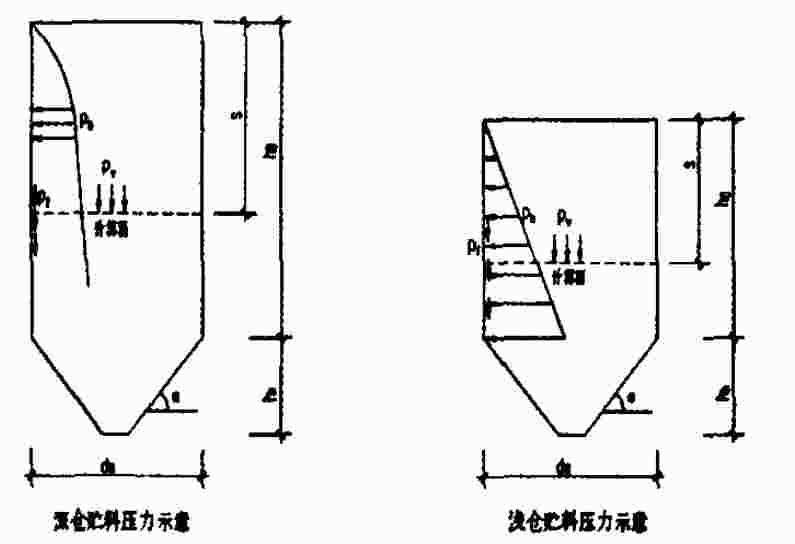
\includegraphics[scale=0.5]{bulker-carve.jpeg}
   \bicaption[figure:bulker-carve]{煤仓结构示意图}{煤仓结构示意图}
								{Fig.}{Schematic diagram of Coal bulker}
\end{figure}

\subsubsection*{煤仓的一般结构}
1) 圆形筒仓仓壁厚度$t$一般为:
\begin{equation}
t=\frac{d_n}{100}+100
\end{equation}
其中,$d_n$为筒仓的直径。
最小厚度不小于$100mm$,当直径大于15m的筒仓,壁厚不小于$300mm$。

2) 筒仓的混凝土强度等级不低于C25,
	露天冻融环境条件下混凝土强度等级不低于C30。
	受力钢筋的混凝土保护层厚度不小于$20mm$。

3) 直径大于等于6米的筒仓,仓壁亦为内外双层配筋,
	在地震区必须为双层配筋;仓壁的水平受力钢筋最小配筋率为0.25\%,
	地震地区不小于0.4\%,受力钢筋直径不小于10。
	仓壁的竖向钢筋在仓底以上六分之—仓壁高度范用内应为0.40\%,
	以上为0.3\%,直径不宜小于$10mm$。

4) 仓壁上开侧下料口时,侧洞的宽度和高度均不宜大于大于$1000mm$,
	并采取一下加强措施:\\
    (1)洞口上下每边附加的水平钢筋面积不应小于被洞口切断的
	水平钢筋面积的0.6倍,洞口左右两侧附加的竖向钢筋面积不应小于
	被洞口切断的竖向钢筋面积的0.5倍。\\
    (2)洞口附加钢筋的配置范围:水平钢筋为仓壁厚度的1—15倍范围。
	竖向钢筋为仓壁厚度的1倍范围,且靠近洞口每侧第一排钢筋根数不少于3根。\\
    (3)附加钢筋的锚固长度:水平钢筋每侧超出洞口边50倍的钢筋直径,
	且不小于洞口高度;竖向钢筋每侧超出洞边不小于35倍的钢筋直径。\\
    (4)洞门四角内外侧斜向应配置一根直径不小于16的斜向加强钢筋,
	锚固长度两边各40倍钢筋直径。

	
\section{与本课题的关系/本论文研究内容(???)}


% !TEX TS-program = XeLaTeX
% !TEX encoding = UTF-8 Unicode

\chapter{盲信号处理理论基础}
\label{chap01}

\section{盲信号处理概述}
盲信号处理问题可以粗略地表述为:在一个多输入多输出(MIMO)
系统中,当传输信道特性未知或所知甚少时,从输出端的传感器阵列
或转换器输出信号中,分离或估计出源信号的波形,再或者辨识
系统的数学模型。盲信号处理是随着数字通信和地球物理勘探等行业
的飞速发展,在信号处理领域兴起的一个新的研究方向。其主要任务是
对未知系统,在其输入信号完全未知或者只有很少先验知识的情况下,
仅有其输出信号来重构输入信号或进行系统辨识。

从这个粗略的定义可以看到,盲信号处理与传统信号处理的最大区别
在于它试图利用最少的信息获取最大的收益,它与神经网络中的无师学习
和模式识别中的动态聚类有着紧密的联系。在天线阵列处理、语音增强
和分离、数字通信中码间干扰和多径效应的消除、地球物理勘探建模
(地震反卷积)、超声分析中都有着广泛的用途。(?*?*?)

因为是在缺乏混合系统和/或滤波过程参数的情况下进行源信号参数
估计的,所以盲信号处理看起来似乎有点不可思议,也很难想像能将
源信号完全估计出来。事实上,在缺乏某些先验知识时,是不可能唯一地
确定源信号的,然而在允许一定程度上的不确定性时,对源信号加以估计
则通常是可能的。用数学术语来说,这种不确定性和模糊性可以看做是
对被估计的源信号的任意比例的伸缩、排序或时滞,但它依然保留了
源信号的波形信息。尽管这种不确定性使盲信号处理具有一定的局限性,
但在很多实际应用中它并非关键问题,因为源的大量相关信息蕴含在
源信号的波形中,而不是信号的振幅或者系统输出的排列顺序中。(***)

盲信号处理的问题分为盲辨识、盲反卷积、盲信号分离三类。

\subsection{盲辨识}
盲辨识是仅利用系统的带噪输出来辨识系统数学模型的盲信号处理方法。
盲辨识问题与传统系统辨识问题存在的一个最大的不同是,在传统系统辨识
问题中,通常假设系统输入和系统输出均可进行测量,而盲辨识中系统输入
是不可测量的,这就要求利用新的信号处理方法对系统的带噪输出进行处理,
得到其它信息,以补偿系统输入未知这一缺陷。

通常使用的方法是过采样技术和高阶统计信息理论。
\paragraph*{过采样技术}
是通过对系统输出进行过采样后,输出具有循环平稳特性的信号,并包含着
系统的相位信息,从而为系统模型的建立提供了可能。(***)

20世纪80年代初,Garder发现利用调制信号的循环平稳特性,可应用二阶
统计理论对通信信道的幅值和相位进行恢复(?*?*?),从而引起了人们采用
二阶统计理论对系统进行盲辨识研究的热潮。其实现方法是采用过采样技术,
即在输入信号的一个采样周期内,系统输出被采样若干次,这样得到的输出
信号不但具有循环平稳特性,而包含着系统的相位信息,从而补偿了系统输入
信号未知这一缺陷,可对系统进行盲辨识。过采样技术具有运算量适中,
算法收敛性好,可辨识非最小相位系统等优点,从而引发了人们的广泛关注。(***)

自从Garder提出可应用而阶统计理论对通信信道的幅值和相位进行恢复以来,
过采样技术取得了很大的发展,目前的研究主要集中在有限冲击响应系统
脉冲序列的确定及算法的可辨识行方面。(***)

\paragraph*{高阶统计信息理论}是二阶相关概念的一种自然推广,
是按照一定的方式对观测量进行多次相关。
20世纪80年代初期,Li和Rosenblatt运用高阶统计信息理论
对非高斯系统进行了研究分析,提出了对各类非高斯问题的统一描述,(?*?*?) 
从而使高阶统计信息理论在将近二十年来得到了突飞猛进的发展。
高阶统计信息理论不但能对系统进行辨识,
而且可用于估计系统的相位,即可以用于非最小相位系统的辨识。
其主要缺点是计算累积误差大,数据窗口长,数值计算量大,
且仅适用于非高斯系统。

盲辨识问题时一个极具挑战性的研究课题,牵涉的知识面广。应用
过采样技术对系统进行盲辨识缺乏系统的理论和方法,还处于发展阶段。
而高阶统计信息理论经过多年的发展,取得了很多有益的成果,但主要还
停留在理论研究方面,工程实践应用还比较少。(?*?*?)

\subsection{盲反卷积}
盲反卷积时仅利用系统的带噪输出对系统的输入进行重构,一般假定
系统输入u(t)为独立、同分布、零均值序列,系统模型未知,系统的输出
可以进行测量。
%          ______________                  ________
%输入u(t)  |             |系统带噪输出y(t) |       | ὒ(t)
%———————-->|未知系统模型 |---------------->|滤波器 |-------->
%          |_____________|                 |_______|

    更一般地,传感器测得的信号是源机器滤波和延迟的混叠信号的线性
组合,通常称为卷积混叠。无噪声多通道卷积混叠信号的数学模型可以
用下式表示:
      x(t)=A(z)s(t)=sigm(正无穷->负无穷) A(k)s(t-k)
式中,x(t)和s(t)同为瞬时混叠式;A(k)为未知滤波混叠矩阵,A(z)为
其Z变换;观测信号x(t)是源信号s(t)通过A(k)的卷积混合,所以矩阵
序列{A(k)}又称冲激响应。
    现有的多通道盲反卷积方法大都是仅通过观测信号x(t)估计通道
冲击响应{A(k)},进而恢复源信号。我们可以直接给出盲反卷积(盲均衡)
模型:
      y(t)=sigm(k 负无穷->正无穷)W(k)x(t-k)=W(z)x(t)
其中,y(t)为均衡输出矢量;W(z)称为均衡器,W(k)为均衡器系数矩阵。

实际进行盲反卷积的算法有:

\paragraph*{H-J算法的扩展}
这类算法是瞬时混叠盲源分离H-J网络训练算法的直接推广。针对反馈
分离网络和卷积混叠模型,卷积混叠信号的反馈分离网络输出为
    xxxxxxxxxxxxxxxxxxxxxxxxxxx
	Platt和Faggin为这类网络确定了用来进行优化的理论准则————最小
输出功率原理,即当独立分量得以分离,则信号的功率达到最小,由此
利用梯度下降法得到该网络的训练公式,它恰好是H-J算法的推广,公式为:
          xxxxxxxxxxxxxxxxxxxxxxxxxxxxxxxxxx
\paragraph*{累积量算法的扩展}
这是一种基于互累积两消失的自适应盲反卷积算法。该算法利用了
盲源分离的经验公式,直接将盲源分离的情况扩展到盲反卷积。公式在形式
上和扩展的H-J方法类似,而H-J公式中的非现行函数用四阶互累积量xxxx
xxxxxxxxxxxxx代替,训练公式为:
     xxxxxxxxxxxxxxxxxxxxxx
\paragraph*{信息理论算法扩展}
对瞬时混叠信号模型,Infomax方法是较成功的盲源分离方法之一。
Torkkola将Infomax算法推广到卷积混叠的情况,得到了一个局部训练
算法(仅有两个源的情况)。该算法通过因果滤波器最大化输出熵最小化
两个输出之间的互信息,基于最大信息传输原理,可以得出直接滤波器
零延迟权系数,直接滤波非零延迟权系数和反馈交叉滤波权系数的训练
公式。而对于更一般的卷积混叠情况,Lee给出了反卷积系统滤波器权系数
的公式:
    xxxxxxxxxxxx
	xxxxxxxxxxxx
	Lambert在他的博士论文中,发展了FIR滤波器多项式代数理论,
并通过仿真实例表明该理论是解决多通道盲源分离的一种有效工具。
应用FIR多项式矩阵代数的基本思路是扩展标量矩阵代数到时域的
滤波器矩阵代数(或频域的多项式矩阵)。利用这一理论可以得到频域
扩展的Infomax算法:
      xxxxxxxxxxxxxxxxxxxxxx
其中,H表示复共轭,W为滤波器矩阵,X和u为频率域多传感器信号块。

\subsection{盲源分离}
所谓盲信号分离,亦即盲源分离,是在没有关于混合矩阵的任何先验
知识的情况下,来辨识混合矩阵或回复所有源信号,它撇开了混合矩阵A的
特性,而只利用接受信号所携带的信息,这种盲方法的性能在本质上将不受
传输模型误差或阵列误差的影响。

盲源分离和所谓独立分量分析(Independent Component Analysis, ICA)
有着非常密切的联系,很多时候,两个名称甚至混用,关于此部分内容,
将在下一章详细介绍。
































\section{盲信号处理历史和现状}
盲源分离(Blind Source Separation, BSS)是指在不知道源信号
和传输通道的参数的情况下,根据输入源信号的统计特性,仅由
观测信号恢复出源信号各个独立成分的过程。现在所指的
盲源分离通常是对观测到的源信号和的线性瞬时混叠信号进行
分离。(***)

在考虑到时间延迟的情况下,观测到的信号应该是源信号和通道
的卷积,对卷积混叠信号进行盲分离通常称为
盲反卷积(Blind Deconvolution, BD) (***)
(张发启 等 盲信号处理及应用 P1)

对含有未知分布噪声的混叠信号进行盲源分离在当前仍然有困难,
上述两种方法现在一般都没有考虑其影响。除了上述的线性瞬时
混叠和卷积混叠外,实际情况中,更一般的情况是非线性的混叠。

较早进行盲源分离方法研究的是Herault和Jutten,他们提出了
一种类神经元分离的方法:基于反馈神经网络,通过选取奇次
的非线性函数构成Hebb训练,从而达到盲源分离的目的(?*?*?)
该方法不能完成多于两个混叠信号的分离,这是因为非线性函数
的选取具有随意性,并且缺乏理论解释。(?*?*?)

Tong和Liu分析了盲源分离问题的可分离性和不确定性,并给出
了一类基于高阶统计的矩阵代数特征分解方法。(?*?*?)
Cardoso提出了基于高阶统计的联合对角化盲源分离方法,
并应用于波束形成。(?*?*?)
Common系统地分析了瞬时混叠信号的盲源分离问题,并明确了
独立分量分析(Independent Component Analysis, ICA)
的概念(?*?*?),利用可以测度源信号统计独立性的Kullbak-
Leibler准则作为对比函数,通过对概率密度函数的高阶近似,
得出用于测度信号各分量统计独立的对比函数,并由此给出一类
基于特征分解的独立分量分析方法。(?*?*?)
Sejnowski和Bell基于信息理论,通过最大化输出非线性节点
的熵,得出一种最大信息传输的准则函数,并由此导出一种
自适应盲源分离和盲反卷积方法(Infomax),当该方法中
非线性函数的选取逼近源信号的概率分布时可以较好地恢复出
源信号。该算法只能用于源信号峭度(Kurtosis)大于某一值的信号
的盲分离,所以它对分离线性混叠的语音信号非常有效。(?*?*?)
Amari和Cichocki基于信息理论中概率密度的Gram Charlier
展开利用最小互信息(Minimum Mutual Information, MMI)准则函数
得出一类前馈网络的训练算法,可以有效分离具有负峭度的源信号,
该类算法具有等变(equivariant)特性,即不受混叠矩阵的影响。(?*?*?)
Hyvӓrinen基于源信号非高斯性测度(或峭度),给出了一类
定点(Fix-point)训练算法,该类算法可以提取单个具有正或负
峭度的源信号。(?*?*?)

在对线性瞬时混叠信号盲源分离方法进行研究的同时,人们对
卷积混叠信号盲分离————盲反卷积方法也进行了研究。
Platt和Faggin将H-J算法推广到具有时间延迟的卷积混叠
情况。(?*?*?)
Yellin和Wensten给出了基于高阶累积量和高阶谱多通道
盲反卷积方法,通过递归特征分解可以同时进行盲系统参数辨识
和盲反卷积。由于用到高阶累积量和需计算高阶谱,该方法
所需计算量极大。(?*?*?)
Thi和Jutten同样利用四阶累积量或四阶矩函数,给出了
卷积混叠信号盲分离的自适应训练方法。(?*?*?)
K. Tokkola 提出了一个反馈网络结构,将Infomax算法
推广到更广泛的情况,即具有时间延迟的源的混叠或卷及混叠
信号的盲分离。(?*?*?)
Lee和Bell将基于信息最大传输或最大似然算法得出的
盲源分离算法变换到频率域,并利用FIR多项式技术进行
盲反卷积。(?*?*?)

最近人们已经开始研究存在噪声的混叠和非线性混叠信号
信号的盲分离问题。非线性盲分离比线性情况的分离难度更大。
较早涉及非线性混叠信号盲分离的是Burel,他用一个两层
感知器和基于误差向后传输思想的无监督训练算法,通过梯度
下降算法优化统计独立的测度函数,得到一种盲分离算法。
该算法可以用于非线性混叠信号的盲分离。(?*?*?)
1996年Parra提出一类前向信息保持非线性结构映射网络,
通过最小化互信息,减小输出各分量间的剩余度,从而可以
得到非线性独立成分。(?*?*?)
Pajunen, Hyvӓrinen和Karhunen用
自组织映射(Self Organization Map, SOM)从非线性混叠信号
中恢复源信号,该算法可以不考虑非线性混叠的形式,但其网络
复杂性呈指数增长且在分离连续源时存在严重的插值误差。(?*?*?)
Yang和Amri利用两层感知器网络结构,通过最大熵和最小互信息
作为刻度独立的代价函数,提出了信息向后传输的训练方法。
当合理选择非线性函数时,该算法可以分离出一些特定
非线性混叠的源信号。(?*?*?)
Taleb和Jutten提出了一种非线性混叠信号盲分离算法,可以
对被称为后非线性混叠的信号进行盲分离。
由于存在噪声的信号分离是困难的,因此以上方法都没有考虑
噪声的影响。因此有人把带噪声的信号混叠看做一种非线性的,
所以现有的一些带噪声混叠的盲分离方法都是利用非线性方法实现的。
Moulines和Cardoso利用逼近最大似然方法进行带噪声混叠信号
的盲分离和盲反卷积,其中用于处理不完全数据的
期望最大化(Expectation Maximinzing, EM)方法是主要的
数学工具。(?*?*?)
Hyvӓrinen指出,在混叠过程中存在噪声意味着观测数据和源
信号存在非线性关系,他用了独立成分和混叠矩阵的联合最大似然
估计方法。(?*?*?)

在对盲源分离理论上的研究已经取得一定进展之后,人们开始
研究盲源分离训练方法的实际应用。
Lee和Bell将基于信息最大传输或最大似然算法得出的盲源分离
训练算法进行盲反卷积,并用于真实记录的语音信号分离。实验证明,
分离后的语音识别率得到了提高。(?*?*?)
Karhunen和Hyvӓrinen等讲神经网络盲分离算法用于提取图像
特征和分离医学脑电波信号。(?*?*?)
Makeig, Jung和Bell等用盲源分离方法将从
脑电(electro-encephalo-graphic, EGG)信号中记录的与事件相关
的相应数据分解为与传感器数量相等的成分。(?*?*?)
Mackeown等还将ICA用于分析核磁共振成像数据集。(?*?*?)
Sahlin和Broman在移动通信的手机中增加一概麦克风,用信号
分离算法改善通信中信号传输之前的信噪比。(?*?*?)
	
国内近期关于盲信号处理理论和应用技术的研究几乎是与国际上
同步的。
凌燮亭利用反馈式神经网络根据Hebbian的学习算法,实现了
近场情况下一般信号的盲分离,并对算法的渐进收敛性和实现信号
分离状态的稳定性进行了讨论。(?*?*?)
何振亚在基于特征分析、高阶谱的盲源分离鹤盲反卷积方法研究中,
提出了一系列新的基于高阶统计和信息理论的判据和算法。在盲系统
参数估计和盲波束形成等方面也取得了很多很好的研究成果。(?*?*?)
最近胡光锐也开始盲语音分离的研究,并提出了基于高斯混合模型
概率密度估计的语音分离方法。


% !TEX TS-program = XeLaTeX
% !TEX encoding = UTF-8 Unicode

\chapter{独立分量分析}
\label{chap02}
\section{盲源分离}

\subsection{盲源分离问题的提出}
盲源分离\ucite{AAPO01}是指:假设由几个物理对象或物理源发出的一组信号,
物理源也可以是发射无线电波的移动电话,可以是同一房间讲话的人,也可以是发出电信号的不同脑区。
同时假设存在多个位于不同位置的传感器或接收机,每个传感器可以分别以不同的权重记录各物理源信号的某种混合,
可能为线性,也可能为非线性组合。

为了更简单地描述此问题,假定有三个信号源,同时有三个传感器获取的三个观测信号。
记观测信号为$x_1(t), x_2(t) \,\mbox{和}\, x_3(t)$,它们是所记录的信号在$t$时间点处的幅值;
记原始信号为$s_1(t), s_2(t)\,和\,s_3(t)$。
于是$x_i(t)$是$s_i(t)$的加权和,而权系数与于源和传感器之间的距离有关:

\parbox{10cm}{
\begin{eqnarray*}
x_1(t)=a_{11}s_1(t)+a_{12}s_2(t)+a_{13}s_3(t) \\
x_2(t)=a_{21}s_1(t)+a_{22}s_2(t)+a_{23}s_3(t) \\
x_3(t)=a_{31}s_1(t)+a_{32}s_2(t)+a_{33}s_3(t) \\
\end{eqnarray*}
}\hfill
\parbox{3cm}{\begin{eqnarray} \label{bss_compose}\end{eqnarray}}

式中,$a_{ij}$是常值系数,表示混合的权重。
因为不可能了解物理混合系统的全部特性(这通常是极其困难的),$a_{ij}$是未知的。
同样源信号$s_i$也无从得知,而要解决的问题这在于此:因为对它们进行直接记录是不可行的。

此问题就是要利用混合量,如$x_1(t)$, $x_2(t)$和$x_3(t)$找出原始信号,这就是盲源分离(BSS)问题。
盲意味着对原始信号和组合组合规律所知甚少。

在假定混合系数$a_{ij}$具有足够的差异时,混合系数构成的矩阵是可逆矩阵。
因此存在一个矩阵$W$以元素$w_{ij}$为系数,使用它可以分离出源信号$s_i$:

\parbox{10cm}{
\begin{eqnarray*}
s_1(t)=w_{11}x_1(t)+w_{12}x_2(t)+w_{13}x_3(t) \\
s_2(t)=w_{21}x_1(t)+w_{22}x_2(t)+w_{23}x_3(t) \\
s_3(t)=w_{31}x_1(t)+w_{32}x_2(t)+w_{33}x_3(t) \\
\end{eqnarray*}
}\hfill
\parbox{3cm}{\begin{eqnarray}\label{bss_slover} \end{eqnarray}}

如果公式(\ref{bss_compose})中的系数$a_{ij}$已知,将它们形成的矩阵求逆即可得到矩阵$W$。

\subsection{基于独立性的源分离}
估计公式(\ref{bss_slover})中的系数$w_{ij}$应该使用具有普遍适应性的方法,
以便适合各种不同的场合,可以给最开始提出的为多元数据寻找一个好的表示法问题提供一种答案。
但是此处只能使用非常一般的统计性质,因为$x_1, x_2, x_3$是全部的观测。
此处还希望找到一个矩阵$W$,使得可以用源信号$s1$, $s2$, $s3$给出这个好的表示法。

找到上述问题的一个非常简单的求解方式,仅通过考虑信号的统计独立性\ucite{AAPO01}就可以。
事实上,在信号是非高斯的情况下,那么只需确定系数$w_{ij}$,使得信号:\\
\parbox{10cm}{
\begin{eqnarray*}
y_1(t)=w_{11}x_1(t)+w_{12}x_2(t)+w_{13}x_3(t) \\
y_2(t)=w_{21}x_1(t)+w_{22}x_2(t)+w_{23}x_3(t) \\
y_3(t)=w_{31}x_1(t)+w_{32}x_2(t)+w_{33}x_3(t) \\
\end{eqnarray*}
}\hfill
\parbox{3cm}{\begin{eqnarray}\label{bss_slover} \end{eqnarray}}

是统计独立的即可。信号$y_1$,$y_2$和$y_3$等同于(或者说一个信号可能是另一个信号乘以一个标量的比例常数)
原始信号$s_1$, $s_2$和$s_3$只需要它们是统计独立的。

事实上,我们就可以估计出信号所对应的系数矩阵W,从而得到源信号(这些信号是用后文提到的FastICA算法估算出来的),
使用的仅仅是统计独立性的信息。
Endolith提供了一个使用FastICA分离语音信号的示例\ucite{FastICA-Sound}。
而估计得到的信号确实等于我们用于产生混合信号的源信号。
而在源分离的问题中,原始信号就是数据集的“独立成分”。


\section{独立成分分析}
\subsection{定义}
前面已经看到,盲源分离问题实际上是寻找一个线性表示,使得此种表示对应的成分统计独立。
在实际情形下,独立性是先验的,找到一个其成真正独立的表示一般是不可能的,
实际需要做的找到一个表示,使其成分尽可能独立\ucite{AAPO01}。

根据这种思路,即可以对ICA进行简单的定义:

给定对于随机变量的一组观测值$(x_1(t),x_2(t),...,x_n(t))$,其中$t$是时间或者样本标号,
假设它们是由独立成分线性混合而得:
\begin{equation} \label{matrix_reslover}
\left[ \begin{array}{c} 
x_1(t) \\
x_2(t) \\
. \\
. \\
. \\
x_n(t)
\end{array} \right]
=\bm{A}
\left[ \begin{array}{c} 
s_1(t) \\
s_2(t) \\
. \\
. \\
. \\
s_n(t)
\end{array} \right]
\end{equation}
式中,A是某个未知矩阵。
在仅能观察到$x_i(t)$的情况下,独立成分分析所需要做的就是估计出矩阵$\bm{A}$和$s_i(t)$。
注意此处还假定了具有数目相同的独立成分$s_i(t)$的数目与观测变量;
这只是一个为了是问题简化的假设,而不是必须的,当然没有这个假设时,需要使用更为复杂的方式处理。

可以表明,该问题是适定的,
也就是说公式(\ref{matrix_reslover})中的模型可估,而且仅当各成分$s_i$是
非高斯性的,这是一个具体要求。
    
\subsection{如何寻找独立成分}
在除独立性外没有其他任何假设的情况下,仍能从线性混合中估计出独立
成分,这个结论可能让人觉得非常吃惊。那么下面我们试图简要地回答上述情况
为什么是可能的,以及如何实现两个基本疑问。
\paragraph*{仅仅不相关是不够的}:
独立性是比不相关性强得多的性质。
对于盲源分离问题,实际上可以找到信号的许多不同的不相关表示法,
但这些表示未必独立,也未必能将源信号分离出来。
不相关性就其本身而言是不足以分离这些成分的。
这也是主成分分析或因子分析不能分离信号的原因:
它们给出的成分除了不相关外就没有更多信息了。

事实上,利用其它成熟的去相关方法,可以将独立成分的任何线性混合变换成线性不相关成分,
其中的混合变换是正交的。这样,ICA的要点就是估计去相关之后留下的未知正交矩阵。
经典方法和去相关方法一样是基于协方差信息的,所以无法进行这种估计。
    
\paragraph*{非线性去相关是基本ICA方法}:
表达独立性如何强于不相关行的一种说法是,独立性本身就蕴含了\textbf{非线性不相关性}:
若$s_1$和$s_2$独立,那么任何非线性变化$g(s_1)$和$h(s_2)$都是不相关的(在它们之间协方差为零的意义下)。
与此形成鲜明对比的是,对于两个仅仅不相关的随机变量,这样两个非线性变换一般不再具有零协方差。
这样我们可以通过一种更强形式的去相关运算来实现ICA:即,寻找一个表示,使得$y_i$即使通过非线性变化仍然不相关。
这给出了估计矩阵$W$的一个原理:

\textbf{ICA估计原理1}:非线性去相关。寻找矩阵$\bm{W}$,
使得对任何$i \ne j$,成分$y_i$和$y_j$不相关,
而且变换之后的成分$g(y_i)$和$h(y_j)$也不相关,其中,
$g$和$h$是某些适当的非线性函数。

这是一个有效的估计ICA的方法:如果选取适当的非线性函数,的确能使用此方法找到独立成分。
虽然这个原理非常直观,但却存在了一个重要的问题:非线性函数$g$和$h$如何选择?
该问题的答案可以从估计理论和信息论中找到。
估计理论提供了可以估计任何一个统计模型的最为经典的方法:极大似然估计。
信息论可以给出独立性的一些准确度量,如互信息。
利用其中任何一种理论,都能确定出满意的非线性函数$g$和$h$。
    
\paragraph*{独立成分是极大非高斯性成分}:极大非高斯性是另一个非常直观和重要的ICA估计原则原则。
其思路是,根据中心极限定理,非高斯性随机变量之和比原变量更加接近高斯变量。
因此,如果取观测混合变量的一个线性组合$y=\sum b_i x_i$
(因为混合模型是线性的,因此该线性组合同时也是独立成分的一种线性组合),
如果它等于独立成分之一,那么它的非高斯性达到极大。这是因为,如果它确实是两个或更多成分的混合,按中心极限定义,
该混合将更接近高斯分布。这样,相关的原理可以表述为:

	\textbf{ICA估计原理2}:极大高斯性。在y的方差为常数的约束下,球现行组合
	y=sigma-i(bi*xi)非高斯性的局部极大值。每个局部极大值给出一个独立成分。
    
	为了在实际应用中度量非高斯性,我们可以使用一些变量,
比方说\textbf{峭度}。峭度是一个高阶累积量,
它是方差的某种推广(利用高阶多项式)。累积量具有一些有趣的代数和统计性质,
这也是它们在ICA理论中起着重要作用的原因。
    
此外,极大非高斯性原理表明了ICA和独立发展技术,
称为\textbf{投影寻踪}的这项技术之间的紧密关系。
在投影寻踪方法里,我们实际上也是寻找具有极大非高斯性的线性组合,
并用于可视化或其它目的。这样独立成分可以解释成投影寻寻踪的方向。
    
当ICA用于提取特征时,极大非高斯性原理也表明了它与在特征提取的神经科学
理论中使用过的\textbf{稀疏编码}之间的紧密关系。
稀疏编码的思路是将数据用成分表示,使得只有很少数量的成分是同时激活的。
在某些情形下,这等价于寻找极大非高斯性成分。

ICA与投影寻中和稀疏编码之间的这些联系,都和一个更为深入的结果有关,
该结果表明,ICA给出了一个\textbf{尽可能结构化}的线性表示。
此论断可以用信息论概念给出其严格的意义,
并且相关结果还表明,独立成分在许多方面比原始随机变量更容易处理。
特别地,独立成分比原始变量更加容易编码(压缩)。
    
\textbf{ICA估计所需信息比协方差更多}:还有很多其它方法也可以估计ICA模型。
这些方法的共同点是,它们考虑了没有包含在协方差矩阵中的某些统计量。
(协方差矩阵包含的是所有xi对之间的协方差)。

利用协方差矩阵,仅可以在通常线性意义下取出各成分间的相关性。
故所有ICA方法都用到了某种形式的\textbf{高阶统计量},高阶特别地
意味着这些信息并未包含在协方差矩阵中。到此为止我们已经遇到过了两类
高阶信息:非线性相关性和峭度。也可以使用其它很多类型的高阶统计量。
    
\textbf{数值方法是重要的}:除了估计原理外,还必须找到一个具体算法,
以实现所需的计算。由于估计原理使用的是非二次的函数,所需要的计算通常
不能用简单的线性代数来表达,因此算法方面的要求可能是很高的。这样,
数值算法就成为ICA估计方法一个不可缺少的组成部分。

数值方法通常是基于某种目标函数的优化。基本的优化方法是梯度法,
而特别有意思的是一个称为FastICA的不动点算法,它似乎是特别为ICA问题
量身定制的,可以充分地挖掘问题的特殊结构。我们可以采用两种方法任意
一个找到用峭度绝对值度量的非高斯性极大解。

\subsection{ICA的约束}
为了确保上面给出的基本ICA模型能被估计,我们必须作出一定的假设和约束。

\textbf{1) 独立成分被假定是统计独立的}
该假设是ICA能够成立的前提,并且,仅仅这个约束已经基本足够保证模型能够被估计,
这就使ICA能作为一个强有力的方法广泛应用于许多不同领域的应用中。

随机变量$y_1,...,y_n$是独立的,从基本概念上理解,是指在$i \ne j$时,
有关$y_i$的取值情况没有提供任何信息给$y_j$的取值。从技术角度,独立可以通过概率密度来定义。
定义$p(y_1,y_2,...,y_n)$为$y_i$的联合概率密度函数,$p_i(y_i)$为$y_i$的边缘概率密度函数
(即只考虑$y_i$本身的概率密度函数)。那么我们说$y_i$是独立的,
当且仅当联合概率密度函数可以因式分解为下面的形式:
\begin{equation}
p(y_1, y_2, ..., y_3) = p_1(y_1)p_2(y_2)...p_n (y_n)
\end{equation}

\textbf{2) 独立成分必须具有非高斯的分布}
高斯分布所有高阶累积量都为零,通常可以直观地说高斯分布“太简单”了,但是估计ICA模型确必需这样的高阶信息。
因此,ICA对于具有高斯变量的观测变量在本质上是不可能实现的。
值得注意的是,为了避免问题变得过于简单,不会在基本模型中假定独立成分的的具体的非高斯分布的样子。

\textbf{3) 为简单起见,我们假定未知的混合矩阵是方阵}
这个假设表示,具有相同个数的独立成分与观测到的混合量的。这个假设在进一步的讨论时的某些情况下是不严谨的。
但这里做该假设可以大大简化估计过程,同时在很多情况下也是够用的,另外得到矩阵$\bm{A}$的估计后,
可以计算它的逆(用$\bm{B}$表示),并简单地通过下式得到其独立成分:
\begin{equation}
\bm{s}=\bm{B}\bm{x}
\end{equation}
这里假定也同时隐含了混合矩阵是可逆的。
如果不是这样,就说明有可以忽略的冗余混合量存在于此,这时矩阵亦不是方阵,
于是独立成分的个数和混合量的个数也不相等了。

在满足上述三个假设(或至少第1和第2两个假设)的前提下,ICA模型是可辨识的,
意指混合矩阵与那些独立成分可以被估计至存在一些平凡不确定性(trivial indetterminacies)的程度。

\subsection{ICA中的含混因素}
在上述定义的ICA模型中,可以发现一些必然的含混因素或者说,不确定性存在其中。
\paragraph*{1) 无法确定独立成分的方差(能量)}
原因是,$\bm{s}$和$\bm{A}$都是未知的,对于某一个源的任意标量乘积
都能通过对$\bm{A}$矩阵对应的列$a_i$除以对应的标量值$a_i$而抵消:
\begin{equation}
\bm{x}=\sum_{i} (\frac{1}{{\alpha}_i} \bm{\alpha}_i)(s_i {\alpha}_1)
\end{equation}
作为推论,对独立成分的幅值进行修正也可以用同样的方式进行。因为上述分类都是随机变量,
假定它们都具有单位方差就是进行修正最自然的方式:$E\{s_i^2\}=1$。
然而在ICA求解方法中归一化约束可以通过调整矩阵A来实现。
不过即使这样,符号的不确定性问题仍然存在:可以通过对某一独立成分乘以-1而不影响模型。
对于绝大多数应用,这种含混因素很可能可以根据问题的性质提前判断,因而并不是问题的关键。

\paragraph*{2) 无法确定独立成分的次序}
这同样是$\bm{s}$和$\bm{A}$均为未知造成的:
公式(\ref{matrix_reslover})中可以把任意一个独立成分作为第一个,也可以任意交换求和式中各项的次序。
公式形式上,就是可以用一个置换矩阵及其逆代入模型,得到$\bm{x=AP^{-1}Ps}$。
原来的独立变量$\bm{s_j}$仍然是$\bm{Ps}$矩阵的元素,而变化的仅仅是次序。
而矩阵$\bm{AP^{-1}}$则是需要通过ICA算法求解的另一个新的混合矩阵。

\subsection{中心化}
不失一般性,所有的混合变量与独立成分具有零均值是一个合理的假定,
如此可以将理论和算法简化到相当好的程度,因此通常被作为一个默认的假设。

实际工程使用中,一般不会满足零均值假设,但是要满足该要求仅需要进行一些预处理,
中心化(centering)这是可以满足这样要求的一种方法。
中心化是在实施ICA之前,使用如下方法对原始的混合信号$\bm{x'}$进行预处理:
\begin{equation} 
\bm{x=x'}-E\{\bm{x'}\}
\end{equation}
同时独立成分的均值也由此成为了零,因为:
\begin{equation}
E\{\bm{s}\}=\bm{A}^{-1}E\{\bm{x}\}
\end{equation}
我们可以放心作为而不用担心影响对混合矩阵的估计,因为通过这样的中心和预处理,混合矩阵仍可保持不变。
在使用中心化数据估计混合矩阵与独立成分之后,
可以通过简单地在独立成分上加$A^{-1}E{x'}$而恢复被减掉的均值。

\subsection{白化}
给定一些随机变量,一件非常直接的事情是通过线性变换将它们转变为线性相互无关的变量。
因此试图采用这样的手段去估计独立变量是一个诱人的想法,这类方法一般称为白化(whitening)或者球面化(sphering),
且经常通过主成分分析(principal component analysis)来实现。
在本节中,我们指出这是不可能的,并讨论ICA和去相关方法的关系。
事实上,白化可作为ICA中一个有用的预处理技术。

不相关是独立性的一个弱化的形式。有一种比不相关略强的特性称为\textbf{白化性}(whitening)。
如果一个零均值的随机向量$\bm{y}$的各分量具有相同的单位方差且相互不相关则称其为白的(或者白化的),
更具体的说是,$\bm{y}$的协方差矩阵(包括相关矩阵)是单位矩阵:
\begin{equation}
E\{\bm{yy}^T\}=\bm{EDE}^T
\label{whitening}
\end{equation}
式中,$\bm{E}$是$E\{\bm{xx}^T\}$的特征向量的正交矩阵,
$\bm{D}$是相应的特征向量的对角矩阵,$\bm{D}=diag(d1,...,dn)$。
这样,就可以利用下面的白化矩阵来实现白化过程:
\begin{equation}
\bm{V}=\bm{ED}^{-1/2}\bm{E}^T
\label{how-whitening}
\end{equation}
式中,只需要通过简单的逐元素开方从矩阵$\bm{D}^{-1/2}$计算得到
$\bm{D}^{-1/2}=diag(d_1^{-1/2},...,d_n^{-1/2})$。
这样得到的白化矩阵记为$E\{\bm{xx}^T\}^(-1/2)$或$\bm{C}^(-1/2)$。
还有一种可以实现白化的方法是主成分分析,也可给出相关的白化矩阵。
白化过程将混合矩阵变换成一个新的矩阵$A$,由式(\ref{whitening})和(\ref{how-whitening})可知:
\begin{equation}
\bm{z=VAs=\tilde{A}s}
\end{equation}
有人也许会希望白化过程能解决ICA问题,
因为白化或者不相关与独立性是相关联的,但事实却并非如此。
不相关的条件比独立要弱,且仅由此估计ICA模型是不够的。为了说明这个问题,
考虑对于z的一个正交变换:
\begin{equation}
\bm{y=Uz}
\end{equation}
由于U具有正交性,可知:
\begin{equation}
E\{\bm{yy}^T\}
=\tilde{\bm{A}}E\{\bm{ss}^T\}\tilde{\bm{A}}^T
=\tilde{\bm{A}}\tilde{\bm{A}}^T=\bm{I}
\end{equation}
因此可以把对混合矩阵的搜索范围限制到正交矩阵的空间中。
可以无须估计原始矩阵的$\bm{A}$的全部$n^2$个参数(矩阵项),
只要估计一个正交混合矩阵$\tilde{\bm{A}}$即可。
一个正交矩阵包含了n(n-1)/2个自由度。
举例来说二维正交变换仅仅由一个角度参量就能确定。在更高维的情况下,
正交矩阵包含的可变参数个数基本上只有任意矩阵参数个数的一半。

因此我们可以说白化过程解决了ICA问题的一半。
由于白化是一个非常简单的标准过程,比任何ICA算法都要简单,
故通过这样的方式降低问题的复杂程度应该是一个不错的想法。
剩下的一半参数必须通过其它手段去估计,其中一些方法在下面的章节中介绍。

在本文的很多章节中,我们都假定数据已经被白化处理过,
并把这样的数据定义为$\bm{z}$。即使在那些并没有明确白化需求的情况,
我们仍然建议进行白化处理,
因为该过程减少了自由参量的个数并明显提高算法的效率,
尤其在高维数据的情况下。
   
\subsection{时间滤波作为预处理}
因为对于时间序列的信号我们可以对它进行任意的线性滤波,
因为它并不改变ICA模型,当然混合矩阵也不会改变,其中有很多滤波方法。
    
\textbf{1) 低通滤波}:是平滑数据的一种方式,经常用来降噪。
基本ICA模型噪声的影响或多或少地被忽略了。
基本ICA模型对于没有很多噪声的数据效果较好,
因此降噪是有用的,有时甚至是必须的。

\textbf{2) 高通滤波和新息}:高通滤波是从数据中去掉缓慢变化的趋势,
其在某些情况下,会增加独立成分的独立性,因此在ICA中可能是有用的。
高通滤波一个更原则性的方法是按照新息(innovation)过程来考虑。
新息比原始过程常常更独立,而且可以认为新息通常比原始
过程非高斯性更强。高通滤波一个可能的问题是,可能会增加噪声。

\textbf{3) 最优滤波}:前面所讲的两种滤波都各自有优缺点。
最优滤波应该增加成分的独立性,同时降低噪声。为达到这一点,
在高通和低通滤波之间做某些折中可能会是最好的办法。
这导致带通滤波,它把最高和最低的频率成分滤掉,剩下中间一个合适的频带。
至于频带怎么选择无法给出一个一般的答案,它应该依赖于数据。
 
除了简单的低通/高通滤波,还可以有更复杂的方法。
例如,可以用(一维)小波变换,也可以其它时频分解方法。
    
\subsection{用PCA进行预处理}
一个对多维数据降维的常用预处理方法是主成分分析(PCA)。
基本上,数据被先行投影到一个子空间:
\begin{equation}
\bm{\tilde{x}=E_n x}
\end{equation}
并保留了最多的信息(在最小二乘的意义上)。
这样做的好处有使混合矩阵成为方阵以及降噪和防止过学习等。

% !TEX TS-program = XeLaTeX
% !TEX encoding = UTF-8 Unicode

\chapter{分离效果的评价标准}

\label{chap03}

在使用独立成分分析算法产生了几组独立成分之后,需要将各组独立成分
与怀疑为影响因素的因子进行比较,考察它们之间的关系。可以使用的方法
有相关系数、互信息、灰色系统理论等。
 
\section{相关系数}
在概率论和统计学中,\textbf{相关(Correlation)},
显示两个随机变量之间线性关系的强度和方向。
在统计学中,相关的意义是用来衡量两个变量相对于其相互独立的距离。
在这个广义的定义下,有许多根据数据特点而定义的用来衡量数据相关的系数。

对于不同数据特点,可以使用不同的系数。
最常用的是\textbf{皮尔逊积差相关系数}。
其定义是两个变量协方差除以两个变量的标准差(方差的平方根)。
\begin{equation}
\rho_{X,Y} = {\mathrm{cov}(X,Y) \over \sigma_X \sigma_Y} 
           = {E((X-\mu_X)(Y-\mu_Y)) \over \sigma_X\sigma_Y}
\end{equation}
其中,$E$是\textbf{数学期望},$cov$表示\textbf{协方差}。

因为$\mu_X = E(X)</math>, <math>\sigma_X^2 = E(X^2) - E^2(X)$,
同样地,对于$Y$,可以写成
\begin{equation}
\rho_{X,Y} = 
       \frac{E(XY)-E(X)E(Y)}
            {\sqrt{E(X^2)-E^2(X)}~\sqrt{E(Y^2)-E^2(Y)}}
\end{equation}
当两个变量的标准差都不为零时,相关系数才有定义。
从柯西-施瓦茨不等式可知,相关系数的绝对值不超过1。
当两个变量的线性关系增强时,相关系数趋于1或-1。
当一个变量增加而另一变量也增加时,相关系数大于0。
当一个变量的增加而另一变量减少时,相关系数小于0。

当两个变量独立时,相关系数为0.但反之并不成立。 
这是因为相关系数仅仅反映了两个变量之间是否线性相关。
比如说,$X$是区间$[-1, 1]$上的一个均匀分布的随机变量。
$Y$ = $X^2$。 那么$Y$是完全由$X$确定。因此$Y$ 和$X$是不独立的。
但是相关系数为0。或者说他们是不相关的。
当$Y$和$X$服从联合正态分布时,其相互独立和不相关是等价的。

当一个或两个变量带有测量误差时,他们的相关性就受到削弱,
这时,\textbf{反衰减性(disattenuation)}是一个更准确的系数。


\section{互信息}
互信息是一组随机变量的成员具有的该集合中其他随机变量的信息的量度。(***)

\subsection{使用熵的定义(***)}
可以利用熵,
将$n$个(标量)随机变量$x_i, i=1,\cdots,n$之间的互信息$I$定义为:
\begin{equation} \label{mutual_info_defination1}
I(x_1, x_2,\cdots ,x_n)=\sum^n_{i=1} H(x_i)-H(\bm{x})
\end{equation}
式中,$\bm{x}$是包含所有$x_i$的那个变量。

互信息可以像熵一样解释成代码长度。
$H(x_i)$这些项给出了当$x_i$这些变量各自单独编码时的码长,
而$H(\bm{x})$给出了当$x$作为一个随机向量即
所有分量都编码在同一个代码中时的码长。
这样,互信息表明了,通过对整个变量进行编码,
相对于对单个分量分别编码所获得的码长的减少量。
一般而言,对整个向量编码会得到更好的代码。
然而,如果$x_i$之间相互独立,它们都不给出对方的信息,
这时我们只需对各个变量分别单独编码,而不增加码长。

\subsection{使用Kullback-Leibler散度的定义(***)}
换另一种观点。利用所谓的Kullback-Leibler散度,
可以把互信息解释成一个距离。
两个$n$维概率密度函数$p^1$和$p^2$之间的Kullback-Leibler距离定义为:
\begin{equation}
\delta(p^1, p^2) = \int p^1(\xi) log \frac{p^1(\xi)}{p^2(\xi)}\,d\xi
\end{equation}
Kullback-Leibler距离可以看成两个概率密度之间的一种距离,
因为它总是非负的。它等于零,当且仅当这两个密度相等。
这是负对数的(严格)凸性和应用经典的Jensen不等式的一个直接推论。
Jensen不等式(***)断言,对于严格凸函数$f$和任一随机变量$y$,
我们有
\begin{equation}
E\{f(y)\} \ge f(E\{y\})
\end{equation}
取$f(y)=-log(y)$,并假设$y=p^2(x)/p^1(x)$,
其中$x$具有由$p^1$给出的分布。这时我们有:
\begin{multline}
\delta(p^1, p^2) = E\{-log \frac{p^2(x)}{p^1(x)} \} 
	= \int p^1(\xi)\{-log \frac{p^2(x)}{p^1(x)} \} 
    \ge f(E\{y\}) \\ 
    = -log \int p^1(\xi)\{ \frac{p^2(x)}{p^1(x)}\}\,d\xi
    = -log \int p^2(\xi)\,d\xi = 0
\end{multline}
进而,在Jensen不等式中等号成立当且仅当$y$是常数。
在这种情况下,它是常数,当且仅当这两个密度相等,
因而,我们证明了前面宣称的Kullback-Leibler散度的性质。

然而,Kullback-Leibler散度并不是一个真正的距离量度,因为它不是对称的。

为了在这里应用Kullback-Leibler散度,
我们将从考虑各随机变量$x_i$之间相互独立的情形开始,
按照独立性的定义,它们的联合概率密度可以分解。
于是,可以用实际密度$p^1=p_x(\zeta)$和分解的密度
$p^2=p_1(\zeta_1)p_2(\zeta_2)\cdots p_n(\zeta_n)$
之间的Kullback-Leibler散度作为$x_i$之间独立性的度量,
其中,$p_i(.)$是$x_i$的边缘密度。事实上,通过简单的代数运算,
可以说明,这个量就等于我们在式(\ref{mutual_info_defination1})中用熵定义的互信息。

Kullback-Leibler散度的定义互信息蕴含了下面的重要性质:
\textbf{互信息是非负的,而它等于零当且仅当各变量相互独立}。
这是Kullback-Leibler散度性质的直接推论。
 

\section{灰色系统理论}
\subsection{概述}
灰色系统理论是由我国原华中理工大学郑聚龙教授在20世纪80年代提出的,
它是用来解决信息不完备系统的数学方法,
它把控制论的观点和方法延伸到复杂的大系统中,
将自动控制与运筹学的数学方法相结合,用独树一帜的方法和手段,
研究了广泛存在于客观世界中具有灰色性的问题。
在短短的时间里灰色系统理论有了飞速的发展,
它的应用已渗透到自然科学和社会经济的许多领域,
显示出这门学科的强大生命力,具有广阔的发展前景。

系统分析的经典方法是将系统的行为看做是随机变化的过程,
用概率统计的方法,从大量数据中寻找统计规律,
这对于统计数据量较大情况下得处理较为有效,
但对于数据量少得贫信息系统的分析则较为棘手。

灰色系统理论研究的是贫信息建模,
它提供了贫信息情况下解决系统问题的新途径。
它把一切随机过程看做是在一定范围内变化的、与时间有关的灰色过程,
对灰色量不是寻找统计规律的角度。通过大样本进行研究,
而是用数据生成的方法。
将杂乱无章的原始数据整理成规律性较强的生成数列后再做研究。
灰色理论认为系统的行为现象尽管是朦胧的,数据是杂乱无章的,
但它毕竟是有序的,有整体功能的,在杂乱无章的数据后面,
必须潜藏着某种规律,灰数的生成,
是从杂乱无章的原始数据中去开拓、发现、寻找这种内在的规律。

\subsection{灰色系统理论的基本概念}
\paragraph*{1. 基本概念}
\subparagraph*{灰色系统}
信息不完全的系统称为灰色系统。
信息不完全一般指:系统因素不完全明确;因素关系不完全清楚;
系统结构不完全知道;系统的作用原理不完全明了。
\subparagraph*{灰数、灰元、灰关系}
灰数、灰元、灰关系是指灰色现象的特征,是灰色系统的标志。
灰数是指信息不完全的数,即只知大概范围而不知其确切值的数,
灰数是一个数集,记为$\otimes$;灰元是指信息不完全的元素;
灰关系是指信息不完全的关系。
\subparagraph*{灰数的白化值}
所谓灰数的白化值是指,令$a$为区间,$a_i$为$a$中的数,
若$\otimes$在$a$中取值,则称$a$为$\otimes$的一个可能的白化值。
\subparagraph*{数据生成}
将原始数据列$x$中得数据$x(k), x=\{x{k}|k=1,2,3,\cdots,n\}$,
按某种要求作数据处理称为数据生成。如建模生成与关联生成。
\paragraph*{2. 累加生成与累减生成}
累加生成与累减生成是灰色系统理论与方法中占据特殊地位的两种数据生成方法,
常用于建模,亦称建模生成。

累加生成(Accumulated Generation Operation,AGO),
即对原始数据列中各个时刻的数据依次累加,从而形成新的序列。

设原始数列为
\begin{equation}
x^{(0)}=\{x^{(0)}(k)|k=1,2,\cdots,n\}
\end{equation}
对$x^{(0)}$作一次累加生成($1-AGO$)
\begin{equation}
x^{(1)}=\sum^k_{i=1}x^{(0)}(i)
\end{equation}
即得到一次累加生成序列
\begin{equation}
x^{(1)}=\{x^{(1)}|k=1,2,\cdots,n\}
\end{equation}
若对$x^{(0)}$作$m$次累加生成(记作$m-AGO$),则有
\begin{equation}
x^{(m)}(k)=\sum^k_{i=1} x^{(m-1)}(i)
\end{equation}

累减生成(Inverse Accmulated Generating Operation,IAGO)是AGO得逆运算,即对生成序列的前后两数据进行差值运算。
\begin{gather}
x^{(m-1)}(k)=x^{(m)}(k)-x^{(m)}(k-1) \notag \\
\cdots\cdots \\
x^{(0)}(k)=x^{(1)}(k)-x^{(1)}(k-1)  \notag
\end{gather}
m-AGO和m-IAGO的关系是:
\begin{equation}
x^{(0)} \quad \xleftrightarrow[m-IAGO]{m-AGO} \quad x^{(m)}
\end{equation}

\subsection{灰色关联分析}
由灰色系统理论提出的灰关联度分析方法,
是基于行为因子序列的微观或宏观几何接近,以分析和确定因子间
的影响程度或因子对主行为的贡献测度而进行的一种分析方法
。灰联度是指事物之间的不确定性关联,
或系统因子与主行为因子之间不确定性关联。
它根据因素之间发展态势的相似或相异程度来衡量因素间的关联程度。
由于关联度分析是按发展趋势作分析,因而对样本量的大小没有太高的要求,
分析时也不需要典型的跟不规律,而且分析的结果一般与定性分析相吻合,
具有广泛的实用价值。
\paragraph*{1. 构造灰关联因子集}
对抽象系统进行关联分析时,首先要确定表征系统特征的数据列。
表征系统有直接法和间接法两种。
直接法指对直接能得到反映系统行为特征的序列,可直接进行灰关联分析;
间接法指对不能直接找到表征系统的行为特征数列。
这就需要寻找表征系统行为特征的间接量,称为映射量,然后用此映射量进行分析。

在灰色系统理论中,确定表征系统特征的序列,并对数据进行处理,
称为构造灰关联因子集。灰关联因子集是灰关联分析的重要概念,
一般来说,进行灰关联分析时,都要把原因因子转换为灰关联因子集。

设时间序列(原始序列)
\begin{equation}
x=\{x(k)|k=1,2, \cdots ,n\}
\end{equation}
常用的转换方法有以下6种: \\
1) 初值化
\begin{equation}
x'(k)=\frac{x(k)}{x(1)}, \quad k=1,2, \cdots, n
\end{equation}
2) 平均值化
\begin{equation}
x'(k)=\frac{x(k)}{\frac{1}{n} \sum_{k=1}^n x(k)}, \quad k=1,2, \cdots, n
\end{equation}
3) 最大值化
\begin{equation}
x'(k)=\frac{x(k)}{\underset{k}{\max} x(k)}, \quad k=1,2, \cdots, n
\end{equation}
4) 最小值化
\begin{equation}
x'(k)=\frac{x(k)}{\underset{k}{\min} x(k)}, \quad k=1,2, \cdots, n
\end{equation}
5) 区间值化 \\
考虑 $x_i=\{x_i(k)|k=1,2, \cdots ,n\}, i=1,2, \cdots ,n$ \\
令 $\max\max X=\underset{i}{\max} \underset{k}{\max} x_i(k)$,\\
则
\begin{equation}
x_i'(k)=\frac{x_i(k)-\min\min X}{\max\max X - \min\min X}
\end{equation}
6) 正因子化 \\
令 $X_{\min}=\underset{k}{\min}x(k)$
\begin{equation}
x'(k)=x(k)+2|X_{\min}|, \quad (k=1,2, \cdots, n)
\end{equation}

\paragraph*{2. 灰关联度的计算公式}
设$x_0=\{x_0(k)|k=1,2, \cdots ,n\}$为参考序列;
$x_i=\{x_i(k)|k=1,2, \cdots ,n\}$为比较序列。则有如下定义:

$x_i(k)$与$x_0(k)$的关联系数为:
\begin{equation}
\xi_i(k)=\frac{\underset{i}{\min}\underset{i}{\min}|x_0(k)-x_i(k)|
				+\rho\underset{i}{\max}\underset{i}{\max}|x_0(k)-x_i(k)|}
			  {|x_0(k)-x_i(k)|
				+\rho\underset{i}{\max}\underset{i}{\max}|x_0(k)-x_i(k)|}
\end{equation}
式中,$\rho$为分辨系数,$\rho$越小分辨率越大,
一般$\rho$的取值区间为$[0,1]$,通常取$\rho=0.5$。

于是,可求出$x_i(k)$和$x_0(k)$的关联系数
\begin{equation}
\xi_i=\{\xi_i(k)|k=1,2,\cdots,n\}
\end{equation}
则关联度定义为:
\begin{equation}
\gamma_i=\gamma(x_0,x_i)=\frac{1}{n}\sum_{k=1}^{n}\xi_i(k)
\end{equation}
灰关联度具有如下特性: \\
1) 规范性
\\
2) 偶对称性
\\   
3) 整体性
   若//,则一般地有
\\  
4) 接近性
   //越小,则//越大,即//与//越接近。

从上述灰关联度的性质(3)可以看出,灰关联度一般不满足对称性,
于是便有了如下满足对称性的灰关联度计算公式:\\
   ①改进关联度法
   
   ②相对变率关联度法
  
   ③斜率关联度法
  
   
   
   3. 关联序
   设参考序列//与比较序列//,其关联度分别为//,按关联度大小排序即为关联序。
   在灰关联分析中,关联序的大小体现了比较因子对参考因子的影响及作用的大小,其意义高于关联度本身的大小。
   需要指出的是,在关联度的分析中,数列的处理方法不同,关联度的大小会发生变化,但关联序一般是不会发生变化的。
也就是说,关联度的大小只是因子之间相互影响、相互作用的外在表现,而关联序才是其实质。

% !TEX TS-program = XeLaTeX
% !TEX encoding = UTF-8 Unicode

\chapter{工程应用}

\label{chap04}

\section{工程背景} 
内蒙古自治区鄂尔多斯市是我国重要的能源基地,
已探明的天然气储量约1880亿立方米,约占全国总储量的三分之一,
已探明的煤炭储量1496亿多吨,约占全国总储量的六分之一。
鄂尔多斯的煤炭资源不仅储量大、分布广,而且品种齐全,
有褐煤、长焰煤、不粘结煤、弱粘结煤、气煤、肥煤、焦煤等,
并且大多埋藏浅,垂直厚度深,易开采。

位于鄂尔多斯市的某煤矿是一座新建的年产千万吨的现代化煤矿。
从2010年开始试运营。试运营开始时已建设完成完善的生产生活设施,
专用铁路也正在建设。
该煤矿同时建设有一个洗煤厂,可以满足整个煤矿最大生产能力时的需求。
同时为了在生产、加工、运输、销售等环节间进行有效的缓存,共建设了10个煤仓。
其中有原煤仓两个,矸石仓两个、块煤仓4个、末煤仓2个。
下图(\ref{figure:xiaoguotu})即为该煤矿的效果图。
\begin{figure}[!htbp]
   \centering
   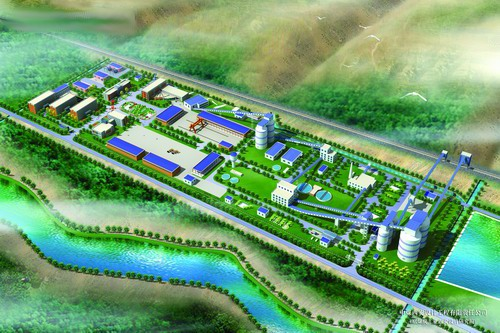
\includegraphics[scale=0.7]{xiaoguotu.jpg}
   \bicaption[figure:xiaoguotu]{厂区效果图}{厂区效果图}
								{Fig.}{Factory renderings}
\end{figure}

矿井生产出的煤炭通过皮带直接运入原煤仓。
经过原煤仓缓存之后,进入洗煤厂进行加工。
经洗煤厂筛选,分选出矸石、块精煤、末煤等,分别进入各自的煤仓。
最后通过各煤仓附属的装载设备,装载到汽车、火车运往各地。

在这些煤仓中,储煤量最大的是两个末煤仓,均可装载2.5万吨煤。
其次是原煤仓,每个装载能力为1万吨。
另外,块精煤仓和矸石仓的装载能力分别为2500吨和1000吨。

根据该煤矿的实际情况,末煤仓的装载能力最大,
日常运营中和使用中装载的煤炭量也最大,因此对地面的压力也最大,
是最需要特别关注的。上图(\ref{figure:xiaoguotu})中,
最大的两个煤仓即为末煤仓。

\section{观测方法}
鉴于煤仓对于安全、有效生产的重要性,在施工过程中和投产使用后,
必须进行沉降观测,以便掌握其沉降情况,及时发现对煤仓运营不利的下沉,
提前采取措施,保证煤仓的安全使用,同时也为今后合理设计提供资料。
本文所提沉降观测仅涉及投产使用后的沉降观测。

本工程的沉降观测采用精密水准测量方法,使用的仪器为徕卡DNA03电子水准仪。

\subsection{水准控制网的布设}
建筑物沉降观测的依据是埋设在建筑物附近的水准点,即基准点。
为了在各基准点之间相互校核并防止因为某个基准点的高程变动而造成基准的错误,
至少埋设三个基准点。
这些控制点应该埋设在建筑物、构筑物基础压力影响范围以外,
避免对沉降原因的判断产生错误;
同时也应该在锻锤、轧钢机、铁路、公路等震动影响范围以外;
并且也要远离地下管道;埋设深度至少要低于冰冻线及地下水位变化范围0.5m。
水准点离开观测点不应太远,以免因为线路过长影响精度。

沉降观测开始时,厂区仍然在进行着频繁的施工建设。
鉴于这种情况,控制网可以按照两级布设。
在厂区外的合适地点,布设第一级控制网,以保证这些点能够稳定,
不受厂区内施工的影响,也不受到采煤的影响。
同时为了观测的方便,在厂区内,布设第二级控制网,
这些控制点的位置应该选择在离各个煤仓位置相对较近、
受施工影响可能比较小、地面条件较稳定的地点。

第一级控制网和第二级控制网要定期进行联测,以检测第二级控制网的稳定性。
联测应该严格按照国家二等水准测量的规范要求进行。
如果第二级控制网发生了变化,要及时采取对控制点进行加固、布设新的控制点、
对控制点高程加常数等措施进行处理,并考虑修正前期煤仓沉降观测值。

(***)国家及行业有关规范标准均规定,
沉降观测点的布设应结合地质情况及建筑物结构特点,
以能全面反映建筑物地基变形特征来确定。
从平面设置考虑, 沉降观测点一般布设在建筑物的四角、转角、
沿外墙 每$10\sim15m$处或每隔$2\sim3$根立柱的柱基上。
从纵向设置考虑,沉降点一般布设在主体的
$± 0.00$以上$0.5m$左右的外墙上较合适,这样观测时立尺、观测均较方便。
建设煤仓时,已经在比较容易到达的地方,预设了四个对称的沉降观测目标点。
通过这四个对称的目标点,既可以检测出煤仓整体的沉降情况,
也可以监测到煤仓可能发生的倾斜情况。

以上所有的第一、第二级控制点,煤仓上的沉降目标点,都需要随时注意保护,
如果发现发生变化或者损坏,需要随时修复并重测,
或者重新布设受损的控制点和目标点。

\subsection{观测时间}
对于煤仓的观测一般采用定期观测的方法。
煤仓刚刚投入使用时,观测的密度需要更加频繁,
随着使用时间的推移,观测密度也随之减小。
在根据周期进行观测的同时,同时也需要注意煤仓的装载量。
如果装载量在短时间内有较大的变化,也需要增加观测,以保证安全。

\subsection{精度选择}
为了能够确保检测出煤仓沉降的变化,需要对观测的精度提出限定。
对观测基准点进行联测时,需要满足国家二等精密水准观测的规范要求,
以保证观测的准确性和可靠性。

在使用基准点对煤仓上的沉降点进行观测时,
对于闭合差、前后视距差等参数的要求严格参考国家二等水准测量的规范要求,
但是并不进行往返测量,
对于其它一些确有困难且并不是特别重要的参数也可以适当放宽要求。
\begin{figure}[!htbp]
   \centering
   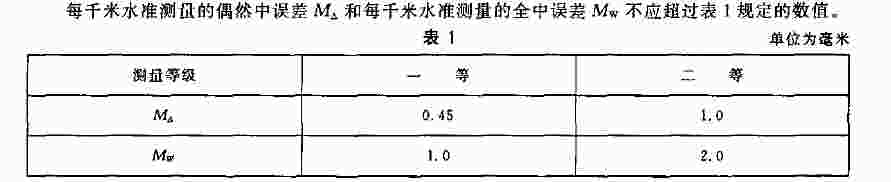
\includegraphics[scale=0.5]{level2requirement1.jpeg}
   \bicaption[figure:error-per-km]{每千米中误差要求}{每千米中误差要求}
								{Fig.}{Error per KM}
\end{figure}

\begin{figure}[!htbp]
   \centering
   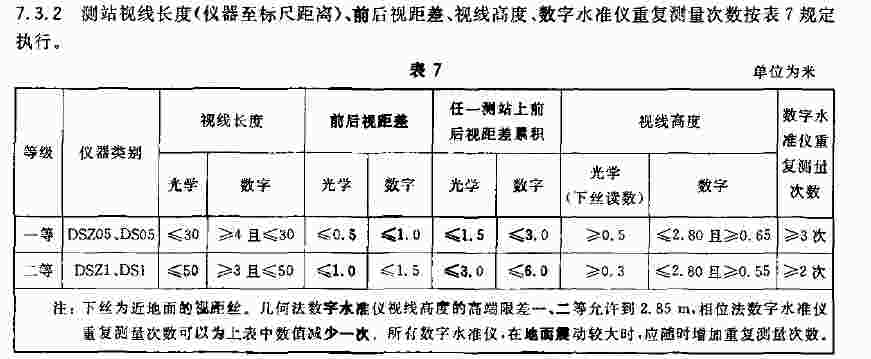
\includegraphics[scale=0.5]{level2requirement2.jpeg}
   \bicaption[figure:line-of-sight]{视线和重复测量要求}{视线和重复测量要求}
						{Fig.}{Line of sight and repeated measurements}
\end{figure}

\begin{figure}[!htbp]
   \centering
   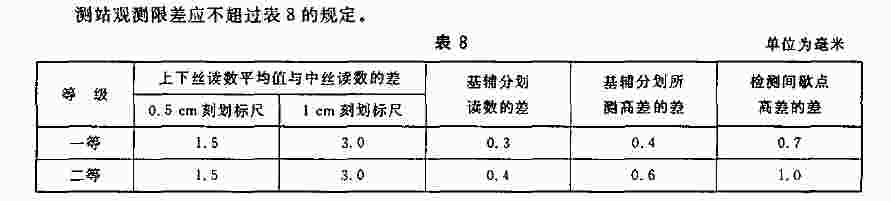
\includegraphics[scale=0.5]{level2requirement3.jpeg}
   \bicaption[figure:b-a-part]{基辅分划读数限差}{基辅分划读数限差}
								{Fig.}{Basic and auxiliary partition}
\end{figure}

\begin{figure}[!htbp]
   \centering
   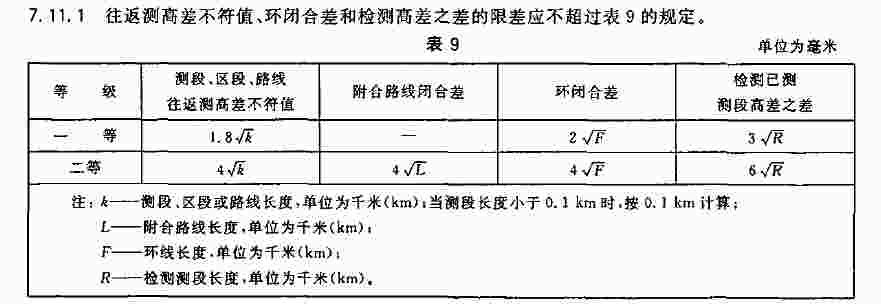
\includegraphics[scale=0.5]{level2requirement4.jpeg}
   \bicaption[figure:go-return]{往返高差不符值、环闭合差、检测高差之差的要求}{往返高差不符值、环闭合差、检测高差之差的要求}
			{Fig.}{Difference of going and forth, Misclosure, Check}
\end{figure}

\newpage
\subsection{预警处理}
当煤仓观测过程中沉降值或者沉降速率超出预警值或者发现煤仓出现倾斜时,
必须立即报告煤仓的使用单位,同时应及时增加观测或着调整观测方案。
同时如果在观测过程中出现煤仓周围进行开挖等作业时,也需要增加观测次数。
另外,如果煤仓周围出现暴雨、爆炸或者地震等特殊情况时,也应该增加观测次数。


\section{数据处理}
03电子水准仪进行,观测的数据也同时存储在电子水准仪中。
内业时,使用LEICA Geo Office软件处理提取出各个观测点的高程值。
将这些观测到的高程值,写入逗号分隔的文本文件(.CSV),
文件中的字段均不加引号,编码使用UTF-8编码。
最后通过使用Python编写的程序,生成HTML格式的各种统计表格以及沉降曲线。

\subsection{原始数据文本数据库}
外业收集的原始数据分为装载量、观测高程、注释和点所属煤仓名等,
将它们分别放置在多个文件中。
建立四个数据文件,分别对应着原煤仓,矸石仓,块精煤仓和末煤仓的沉降数据。
各个文件中,煤仓沉降点名按照煤仓类型统一编号。

1)装载量数据文件的格式为:第一行为观测日期,第二行为观测者姓名,
第三行为数据计算者姓名,
第四行及以下为各个煤仓的装载量(装载量占总装载能力的百分比)。
每个字段均不加引号。
\begin{figure}[!htbp]
   \centering
   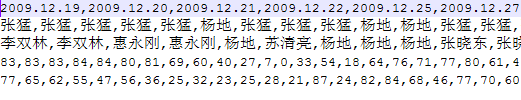
\includegraphics[scale=0.5]{4-heavy-csv.png}
   \bicaption[figure:4-heavy]{装载量文本数据库格式}{装载量文本数据格式}
			{Fig.}{Format of text-database for load}
\end{figure}

高程观测值文件的格式同样也是逗号分隔的文本文件,其格式为:第一行是观测日期,从第二行起是煤仓上各沉降点的高程观测值。
\begin{figure}[!htbp]
   \centering
   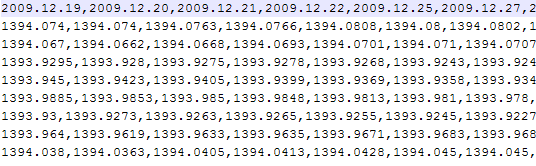
\includegraphics[scale=0.5]{4-level-csv.png}
   \bicaption[figure:4-level]{高程值数据文件格式}{高程值数据文件格式}
			{Fig.}{Format of text-database for leveling}
\end{figure}

注释文件的格式与高程观测值文件的格式完全相同,
但是如果遇到某个数据与高程观测值文件中对应的文件不同,
注释文件中的此数据在生成报表文件时将会作为注释对待。

\newpage
点号文件存储了每个煤仓上沉降点的信息。
第一列是煤仓类型的编号,依次为一号原煤仓、二号原煤仓、一号矸石仓等。
第二列及后面各列是每个煤仓上沉降点的编号。
\begin{figure}[!htbp]
   \centering
   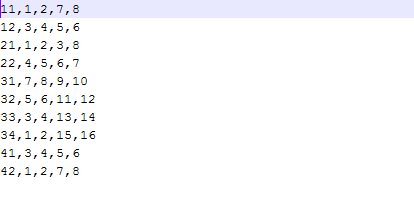
\includegraphics[scale=0.5]{static-csv.png}
   \bicaption[figure:static-csv]{点号数据库格式}{点号数据库格式}
			{Fig.}{Format of text-database for point number}
\end{figure}

\subsection{生成的报表以及图像}
根据观测数据文件,使用Python编程语言编写报表生成程序,
生成了几种需要的报表格式以及沉降曲线。

单点沉降值表,包括序号、时间、本次下沉、累积下沉、高程、
载荷、观测者、计算者、备注共10项。这个表格的每一行表示一次观测。
\begin{figure}[!htbp]
   \centering
   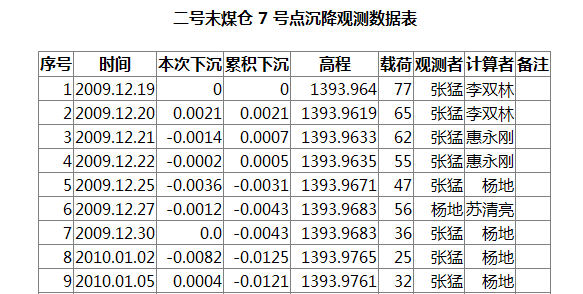
\includegraphics[scale=0.5]{42-7-all.png}
   \bicaption[figure:set-for-single]{单点沉降报表}{单点沉降报表}
			{Fig.}{Report for single point}
\end{figure}

\newpage
煤仓各点高程表,总结煤仓上各点的高程观测值。
\begin{figure}[!htbp]
   \centering
   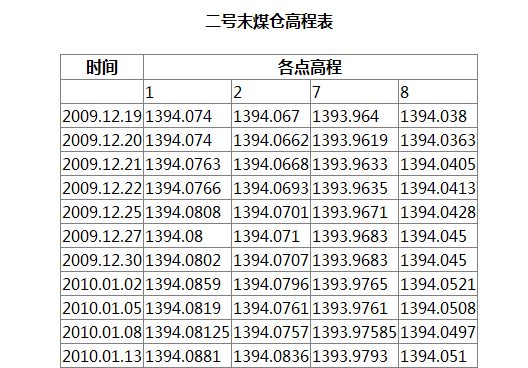
\includegraphics[scale=0.5]{42-new-level.png}
   \bicaption[figure:level-for-bunker]{煤仓上各点高程观测值}
					{煤仓上个点高程观测值}
			{Fig.}{Leveling of points in 1 bunker}
\end{figure}

煤仓各点沉降表,总结煤仓上各点的沉降值。
\begin{figure}[!htbp]
   \centering
   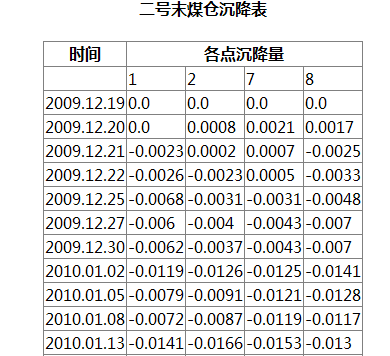
\includegraphics[scale=0.5]{42-settle.png}
   \bicaption[figure:level-for-bunker]{煤仓上各点沉降量}
					{煤仓上各点沉降量}
			{Fig.}{Settlement of points in 1 bunker}
\end{figure}
\newpage

沉降观测阶段总结表模板,根据命令行参数,生成需要提交的阶段总结模板,
经过适当的修改后,提交给委托方。
\begin{figure}[!htbp]
   \centering
   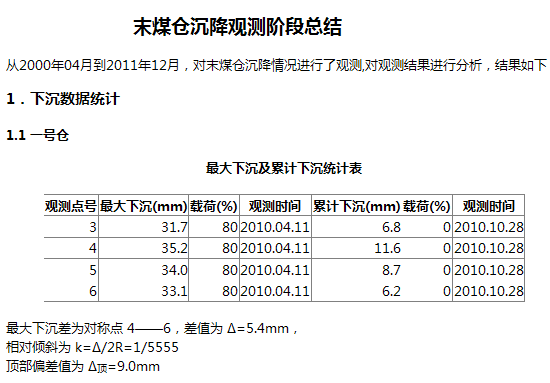
\includegraphics[scale=0.5]{4-paper.png}
   \bicaption[figure:paper]{阶段总结模板}
				    {阶段总结模板}
			{Fig.}{Template for periodic reports}
\end{figure}

沉降曲线图,横轴为从开始测量至最后一次测量的天数;
纵轴正方向为装载量,负方向为各点沉降量。
\begin{figure}[!htbp]
   \centering
   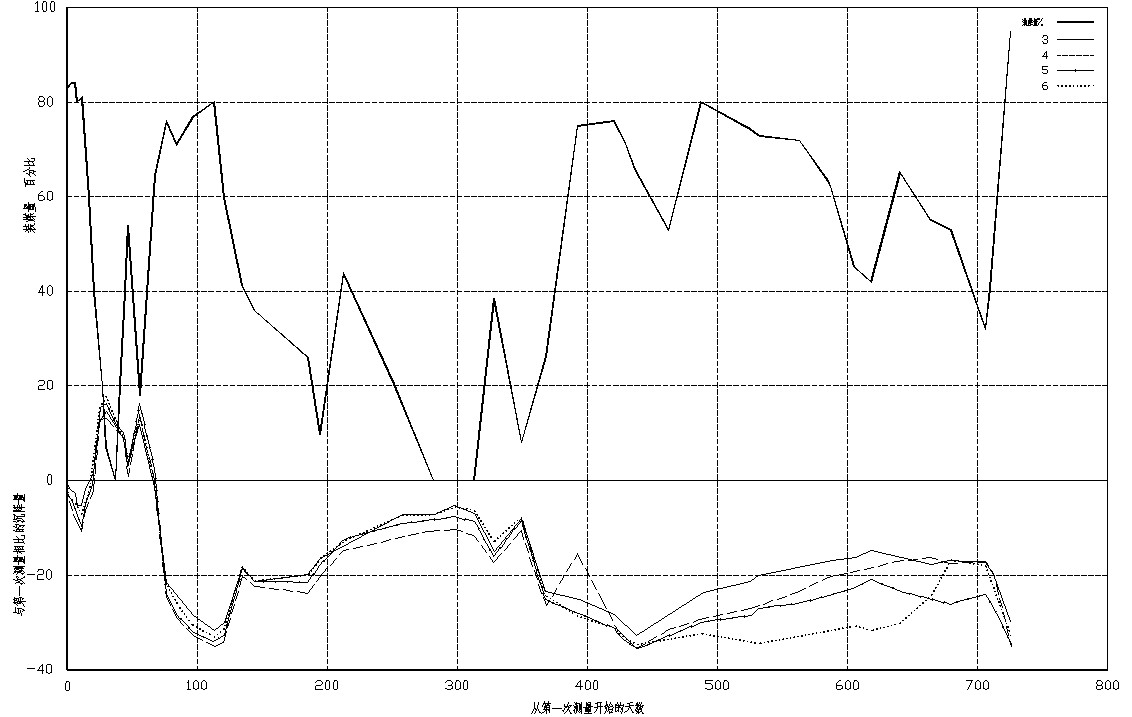
\includegraphics[scale=0.3]{41-plot.png}
   \bicaption[figure:plot-41]{一号末煤仓沉降曲线图}
				    {一号末煤仓沉降曲线图}
			{Fig.}{Curves for settlement fof Powder Bulker No.1}
\end{figure}

\begin{figure}[!htbp]
   \centering
   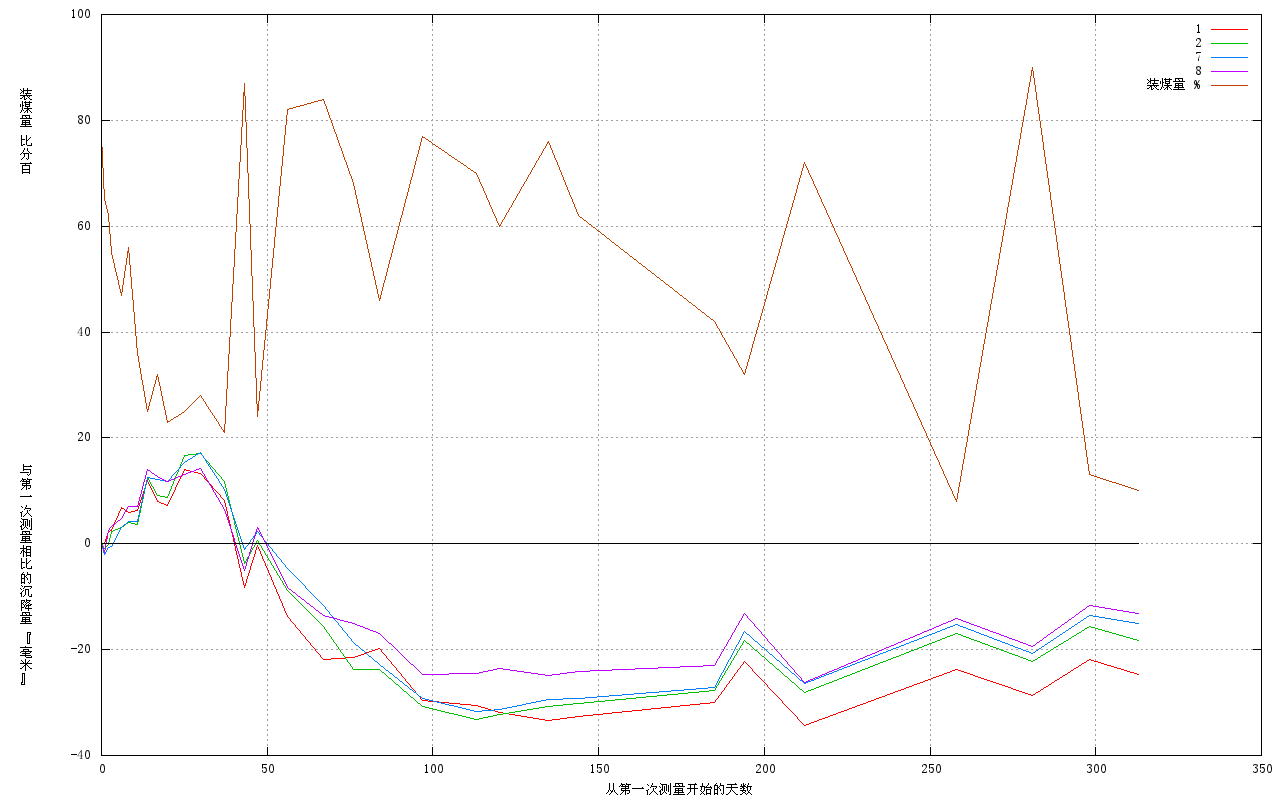
\includegraphics[scale=0.3]{42-plot.png}
   \bicaption[figure:plot-42]{二号末煤仓沉降曲线图}
				    {二号末煤仓沉降曲线图}
			{Fig.}{Curves for settlement of Powder Bulker No.2}
\end{figure}

\section{FastICA}
FastICA是一种流行的高效的独立成分分析算法,
是赫尔辛基理工大学的Aapo Hyvärinen发明。
该算法基于定点迭代方法,并以最大非高斯性作为统计独立性标准。
FastICA也可以导出相应的牛顿迭代方法。

其中一个单元的FastICA算法为(Wikipedia ***):\\
	1. 选择初始向量$W$ \\
	2. 令 $\bm{w}^{+} \quad \leftarrow 
			\quad E\{\bm{x}g(\bm{w^Tx})\} - E\{g'(w^Tx)\}w$ \\
	3. 令 $\bm{w} \quad \leftarrow \quad 
			\bm{w}^{+}/||\bm{w}^{+}||$ \\
	4. 如果未达到收敛要求,继续第2步 \\
此迭代算法求使数据$X$的投影达到最大高斯性的权向量W的方向。
函数$g()$是一个非二次的非线性函数的导数。
例如$g(t)$可是是$f(t)=t^4$的导数。

赫尔辛基理工大学信息和计算机科学实验室的研究人员
基于Matlab和GNU Octave开发了官方FastICA实现,
拥有易用的图形界面和计算功能强大的算法。
除此之外还有R语言、C++、Python等语言的实现。

MDP(Modular toolkit for Data Processing)是
一个基于Python的数据处理框架,
提供了丰富强大的数据处理功能,其中就包括FastICA和PCA。
本文即使用了MDP。

使用FastICA对一组数据进行分析的方法一般有两种:
直接使用FastICA算法,得到和原始数据同样数量的独立成分;
也可以首先使用主成分分析(PCA)对数据进行降维处理,
再使用FastICA进行分析。   

为了评估应用独立成分分析的效果,
可以使用Pearson相关系数、互信息和灰关联度作为评价指标。
计算得到的各独立成分与疑为影响因子之间的
Pearson相关系数、互信息和灰关联度,
根据这些关联性指标分析分离效果以及各种因素对煤仓沉降的影响。

\subsection{直接使用FastICA}
以末煤仓为例,将煤仓上4个点的观测序列分别作为原始信号,
直接使用MDP中的fastica函数进行分析,得出4个独立成分。

MDP中fastica函数原型是:
\begin{lstlisting}[language=Python, basicstyle=\ttfamily]
fastica(x, **kwargs)
\end{lstlisting}
其中的$x$为输入的原始信号,$kwargs$是在分离时使用的参数。\\
可以使用的参数及其默认值为
\begin{lstlisting}[language=Python, basicstyle=\ttfamily]
approach='defl', g='pow3', guess=None, fine_g='pow3', mu=1, 
stabilization=False, sample_size=1, fine_tanh=1, fine_gaus=1,
max_it=1000, max_it_fine=100, failures=5, limit=0.001, 
verbose=False, whitened=False, white_comp=None, white_parm=None,
input_dim=None, dtype=None
\end{lstlisting}
具体每个参数的定义请参考MDP的相应文档(***)。

该处直接使用默认参数,即:
\begin{lstlisting}[language=Python, basicstyle=\ttfamily]
fastica(x)
\end{lstlisting}
如下图像为,使用FastICA之后,根据得到的数据得到的,
观测值的图形见图(\ref{figure:plot-41})和(\ref{figure:plot-42})。

%一号末煤仓使用FastICA后得到的四个独立分量及装载量、气温的图像:
\begin{figure}[!htbp]
   \centering
   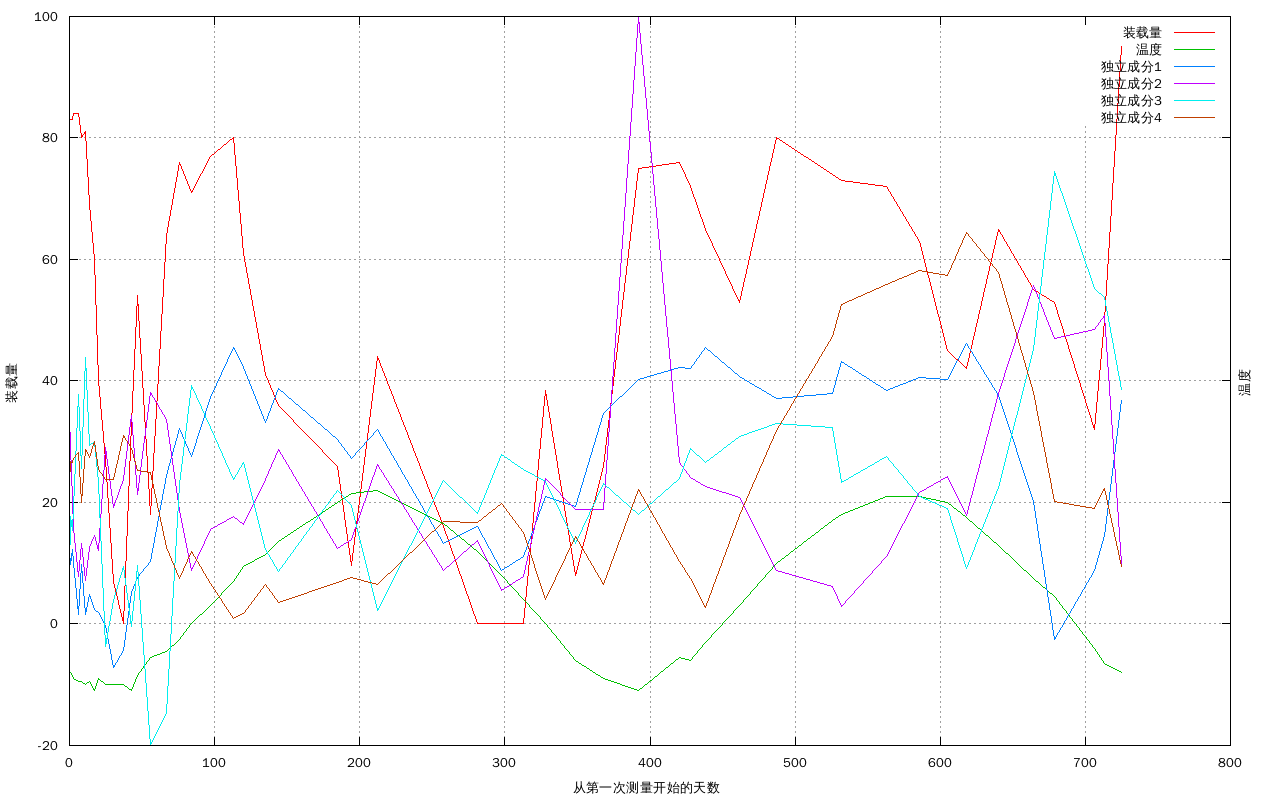
\includegraphics[scale=0.3]{41-ica-plot.png}
   \bicaption[figure:plot-41-ica]{一号末煤仓使用FastICA后得到的四个独立分量及装载量、气温的图像}
				    {一号末煤仓使用FastICA后得到的四个独立分量及装载量、气温的图像}
			{Fig.}{Four IC, Loadage and Temperature for Powder Bulker No.1}
\end{figure}

%二号末煤仓使用FastICA后得到的四个独立分量及装载量、气温的图像:
\begin{figure}[!htbp]
   \centering
   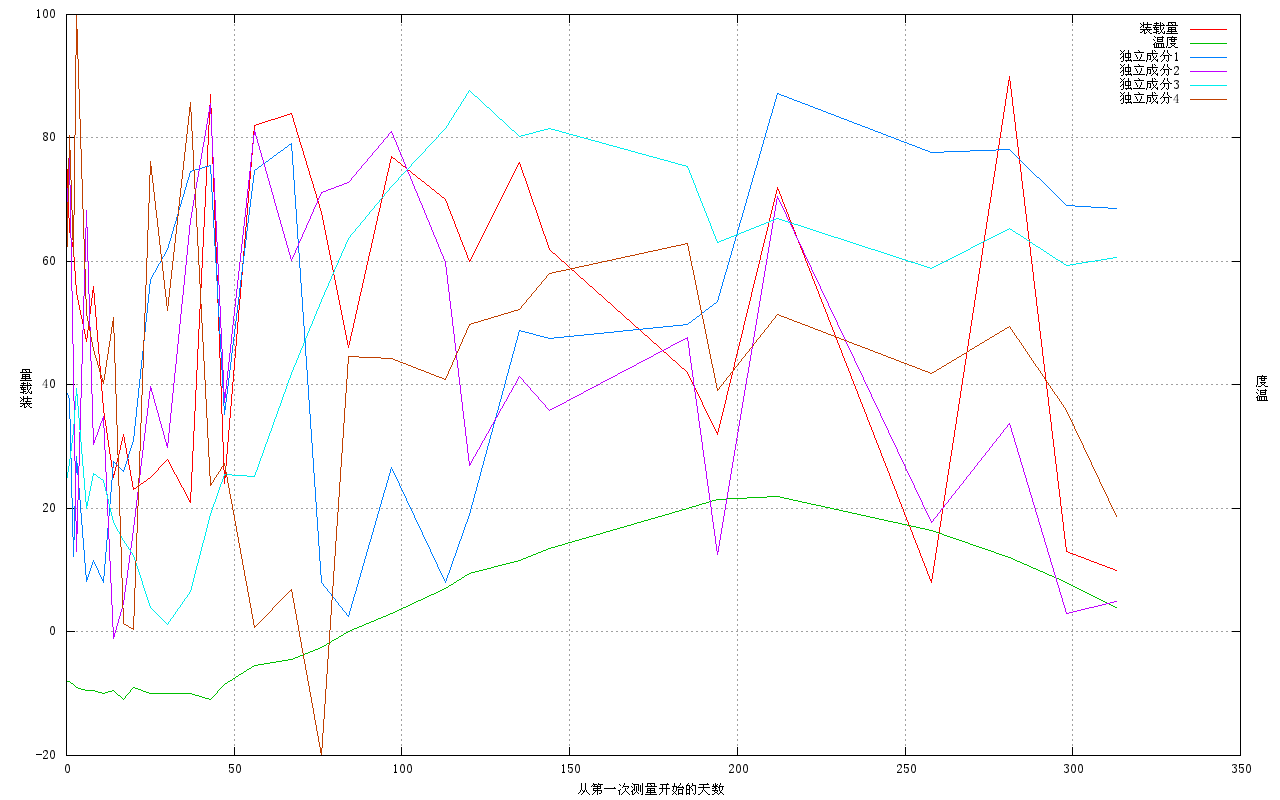
\includegraphics[scale=0.3]{42-ica-plot.png}
   \bicaption[figure:plot-42-ica]{二号末煤仓使用FastICA后得到的四个独立分量及装载量、气温的图像}
				    {二号末煤仓使用FastICA后得到的四个独立分量及装载量、气温的图像}
			{Fig.}{Four IC, Loadage and Temperature for Powder Bulker No.2}
\end{figure}


\subsection{首先使用PCA降维再应用FastICA}
MDP中也带了pca函数,可以用来对信号进行降维。
pca函数的原型是:
\begin{lstlisting}[language=Python, basicstyle=\ttfamily]
pca(x, **kwargs)
\end{lstlisting}
其中,$x$是需要进行主成分分析的信号,
$kwargs$是传递给pca函数的参数,
其可用的参数及其默认值有:
\begin{lstlisting}[language=Python, basicstyle=\ttfamily]
input_dim=None, output_dim=None, dtype=None, svd=False, 
reduce=False, var_rel=1e-12, var_abs=1e-15, var_part=None
\end{lstlisting}
关于具体的使用说明,请参考MDP的文档。
这里我们需要指定输入和输出的信号的维数:
\begin{lstlisting}[language=Python, basicstyle=\ttfamily]
pca(x, input_dim=4, output_dim=3)
\end{lstlisting}
此处我们设定输入的信号维数为4,输出的为3,
以和可能的影响因素的个数相同。
使用PCA对原始信号降维之后,再使用fastica函数获取独立分量。

以下对PCA降维后获得的数据使用fastica之后,画出的图像。
观测值的图形见图(\ref{figure:plot-41})和(\ref{figure:plot-42})

%一号末煤仓使用PCA+FastICA后得到的四个独立分量及装载量、气温的图像:
\begin{figure}[!htbp]
   \centering
   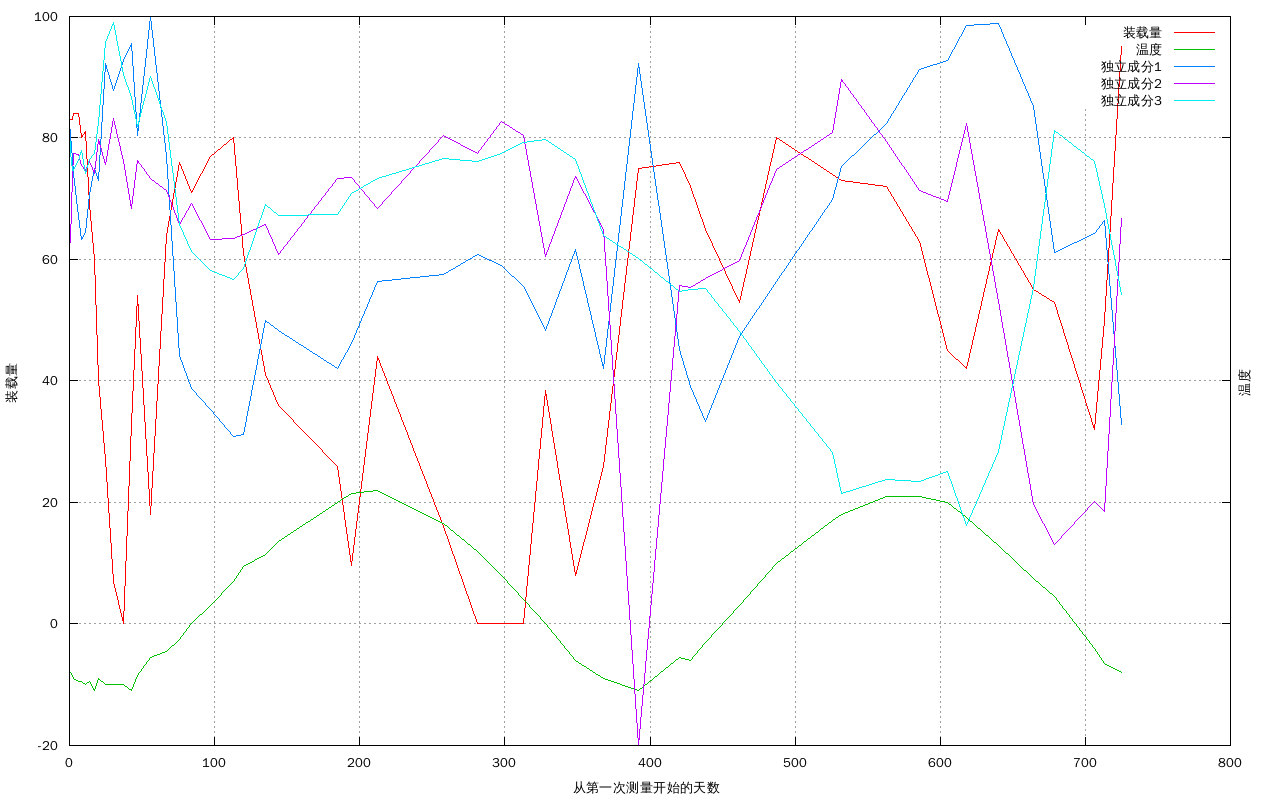
\includegraphics[scale=0.3]{41-pca-plot.png}
   \bicaption[figure:plot-41-pca]{一号末煤仓PCA降维后使用FastICA后得到的四个独立分量及装载量、气温的图像}
				    {一号末煤仓使用PCA降维FastICA后得到的四个独立分量及装载量、气温的图像}
			{Fig.}{Four IC(With PCA first), Loadage and Temperature for Powder Bulker No.1}
\end{figure}

%二号末煤仓使用PCA+FastICA后得到的四个独立分量及装载量、气温的图像:
\begin{figure}[!htbp]
   \centering
   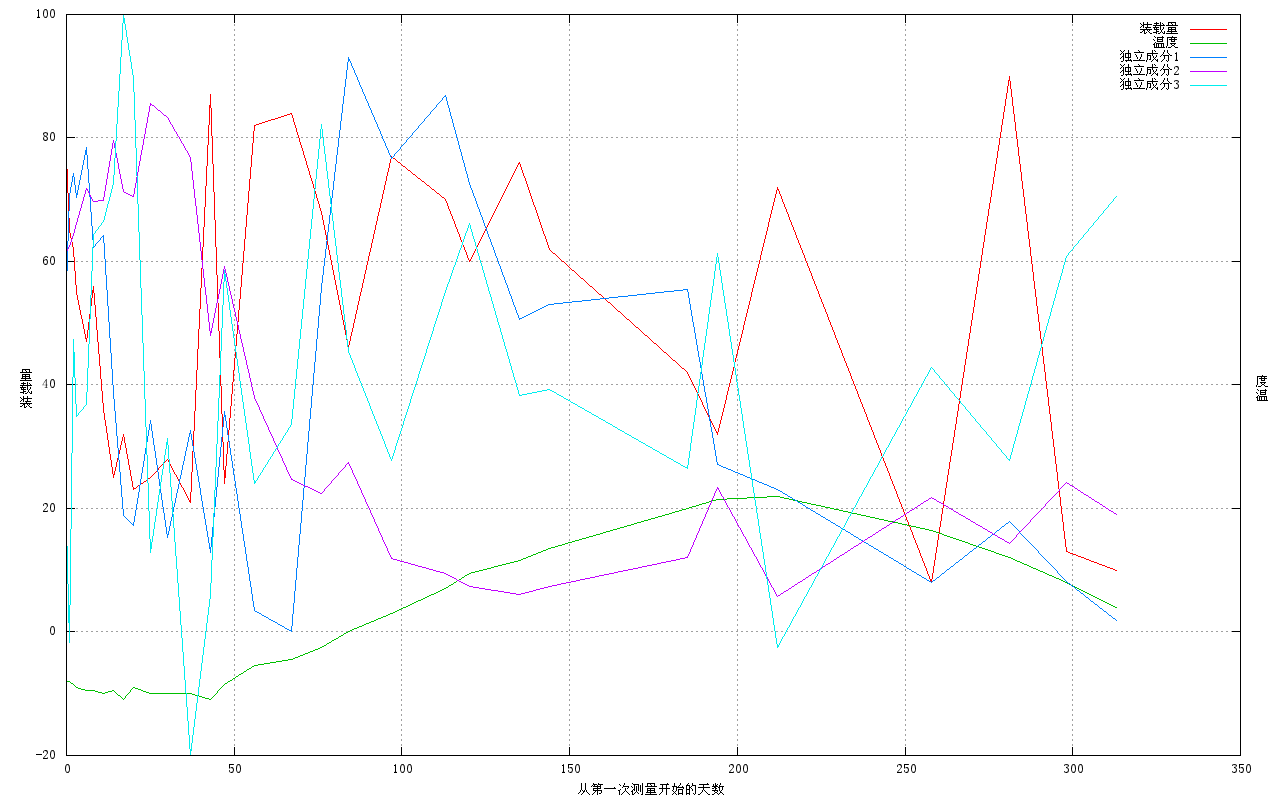
\includegraphics[scale=0.3]{42-pca-plot.png}
   \bicaption[figure:plot-42-pca]{二号末煤仓PCA降维后使用FastICA后得到的四个独立分量及装载量、气温的图像}
				    {二号末煤仓使用PCA降维FastICA后得到的四个独立分量及装载量、气温的图像}
			{Fig.}{Four IC(With PCA first), Loadage and Temperature for Powder Bulker No.2}
\end{figure}

\subsection{各影响因子与所得独立成分的关系}
在根据fastica或者PCA之后的FastICA得到独立成分之后,
为了评估各个独立成分与煤仓装载量、温度变化、经历时间的相互关系,
同时采用Pearson相关系数、互信息、灰关联度作为度量。

%直接FastICA后得到四个独立成分和煤仓装载量之间的相关度量 
\begin{table}[!htb]
\begin{center}
\bicaption{直接使用FastICA得到的独立成分与装载量之间的关系(一号末煤仓)}
			{直接使用FastICA得到的独立成分与装载量之间的关系(一号末煤仓)}
			{Table.}{Relationship between Loadage and ICs from FastICA directly, No.1 of Powder Bulker}
\begin{tabular}{lccclccc}
\toprule
                		& 相关系数     				& 互信息      					&灰关联度 \\
\midrule
  独立成分1     	&  0.31045550206419115       	& 0.94230515613664989   	&    \\
  独立成分2     	&  nan          					& 3.493152145488611e-15   	&    \\
  独立成分3     	&  0.63203026974852217      	& 0.94230515613664989		&    \\
  独立成分4     	&  -0.13494294423250519    	& 0.9423051561366498		&    \\
 \bottomrule
\end{tabular}
\end{center}
\end{table}

\begin{table}[!htb]
\begin{center}
\bicaption{直接使用FastICA得到的独立成分与装载量之间的关系(二号末煤仓)}
			{直接使用FastICA得到的独立成分与装载量之间的关系(二号末煤仓)}
			{Table.}{Relationship between Loadage and ICs from FastICA directly, No.2 of Powder Bulker}
\begin{tabular}{lccclccc}
\toprule
                		& 相关系数     				& 互信息      					&灰关联度 \\
\midrule
  独立成分1     	&  -0.0098565966362569018  	& 0.97325847231868035   	&    \\
  独立成分2     	&  0.64991952670167907		& 0.97325847231868035   	&    \\
  独立成分3     	&  0.27993093051194867      	& 0.9732584723186803		&    \\
  独立成分4     	&  -0.048345889699784657    	& 0.97325847231868035		&    \\
 \bottomrule
\end{tabular}
\end{center}
\end{table}

%直接FastICA后得到四个独立成分和气温之间的相关度量
\begin{table}[!htb]
\begin{center}
\bicaption{直接使用FastICA得到的独立成分与气温之间的关系(一号末煤仓)}
		{直接使用FastICA得到的独立成分与气温之间的关系(一号末煤仓)}
			{Table.}{Relationship between Temperature and ICs from FastICA directly, No.1 of Powder Bulker}
\begin{tabular}{lccclccc}
\toprule
                & 相关系数     						& 互信息      						&灰关联度 \\
\midrule
  独立成分1     &  -0.79715083668276143     	& 0.92753315430712713			&    \\
  独立成分2     &  nan							& 3.3089362752306921e-15		&    \\
  独立成分3     &  -0.0046455198649242432		& 0.92753315430712824 			&    \\
  独立成分4     &  -0.12419823845502126		& 0.92753315430712857 			&    \\
 \bottomrule
\end{tabular}
\end{center}
\end{table}

\begin{table}[!htb]
\begin{center}
\bicaption{直接使用FastICA得到的独立成分与气温之间的关系(二号末煤仓)}
		{直接使用FastICA得到的独立成分与气温之间的关系(二号末煤仓)}
			{Table.}{Relationship between Temperature and ICs from FastICA directly, No.2 of Powder Bulker}
\begin{tabular}{lccclccc}
\toprule
                & 相关系数     						& 互信息      						&灰关联度 \\
\midrule
  独立成分1     &  0.33269827762973381	     	& 0.92753315430712879			&    \\
  独立成分2     &  -0.11181095960366073		& 0.92753315430712746			&    \\
  独立成分3     &  0.84894488520244671		& 0.9275331543071224 			&    \\
  独立成分4     &  0.046542855465477796		& 0.92753315430712779			&    \\
 \bottomrule
\end{tabular}
\end{center}
\end{table}

%直接FastICA后得到四个独立成分和时间之间的相关度量
\begin{table}[!htb]
\begin{center}
\bicaption{直接使用FastICA得到的独立成分与时间之间的关系(一号末煤仓)}
		{直接使用FastICA得到的独立成分与时间之间的关系(一号末煤仓)}
			{Table.}{Relationship between Days and ICs from FastICA directly, No.1 of Powder Bulker}
\begin{tabular}{lccclccc}
\toprule
                		& 相关系数     					& 互信息      					&灰关联度 \\
\midrule
  独立成分1     	&  -0.67039265728626118     		& 0.99999999999824107   	&    \\
  独立成分2     	&  nan          						& 4.0089740251131844e-15   	&    \\
  独立成分3     	&  -0.26336501825181907      		& 0.99999999999824218   	&    \\
  独立成分4     	&  -0.23270816025544519      		& 0.99999999999824252  	&    \\
 \bottomrule
\end{tabular}
\end{center}
\end{table}

\begin{table}[!htb]
\begin{center}
\bicaption{直接使用FastICA得到的独立成分与时间之间的关系(二号末煤仓)}
		{直接使用FastICA得到的独立成分与时间之间的关系(二号末煤仓)}
			{Table.}{Relationship between Days and ICs from FastICA directly, No.2 of Powder Bulker}
\begin{tabular}{lccclccc}
\toprule
                		& 相关系数     					& 互信息      					&灰关联度 \\
\midrule
  独立成分1     	&  0.51625222015459338     		& 0.99999999999824285   	&    \\
  独立成分2     	&  -0.28080031928822285		& 0.99999999999824141   	&    \\
  独立成分3     	&  0.68571871171874499      		& 0.99999999999824307   	&    \\
  独立成分4     	&  -0.113386396661022      		& 0.99999999999824196  	&    \\
 \bottomrule
\end{tabular}
\end{center}
\end{table}

%首先使用PCA降维再使用FastICA后得到三个独立成分和煤仓装载量之间的相关度量
\begin{table}[!htb]
\begin{center}
\bicaption{PCA降维后使用FastICA得到的独立成分与装载量之间的关系(一号末煤仓)}
		{PCA降维后使用FastICA得到的独立成分与装载量之间的关系(一号末煤仓)}
			{Table.}{Relationship between Loadage and ICs from FastICA after PCA, No.1 of Powder Bulker}
\begin{tabular}{lccclccc}
\toprule
                		& 相关系数     					& 互信息      						&灰关联度 \\
\midrule
  独立成分1     	&  0.2635564858132709     		& 0.94230515613664989   		&    \\
  独立成分2     	&  0.3483940146795545			& 0.94230515613664989  		&    \\
  独立成分3     	&  0.62976934113327743			& 0.94230515613664989			&    \\
 \bottomrule
\end{tabular}
\end{center}
\end{table}

\begin{table}[!htb]
\begin{center}
\bicaption{PCA降维后使用FastICA得到的独立成分与装载量之间的关系(一号末煤仓)}
		{PCA降维后使用FastICA得到的独立成分与装载量之间的关系(一号末煤仓)}
			{Table.}{Relationship between Loadage and ICs from FastICA after PCA, No.1 of Powder Bulker}
\begin{tabular}{lccclccc}
\toprule
                		& 相关系数     					& 互信息      						&灰关联度 \\
\midrule
  独立成分1     	&  0.25118155055662922     		& 0.97325847231868035   		&    \\
  独立成分2     	&  -0.36213168393230483		& 0.97325847231868035  		&    \\
  独立成分3     	&  -0.35052673089969216		& 0.97325847231868035			&    \\
 \bottomrule
\end{tabular}
\end{center}
\end{table}

%首先使用PCA降维再使用FastICA后得到三个独立成分和气温之间的相关度量
\begin{table}[!htb]
\begin{center}
\bicaption{PCA降维后使用FastICA得到的独立成分与气温之间的关系(一号末煤仓)}
			{PCA降维后使用FastICA得到的独立成分与气温之间的关系(一号末煤仓)}
			{Table.}{Relationship between Days and ICs from FastICA after PCA, No.1 of Powder Bulker}
\begin{tabular}{lccclccc}
\toprule
                & 相关系数     				& 互信息      			&灰关联度 \\
\midrule
  独立成分1     &  -0.82599874780257931		& 0.92753315430712724   &     \\
  独立成分2     &  0.028941710801729584		& 0.92753315430712802   &     \\
  独立成分3     &  0.063245341965641827		& 0.92753315430712824   &      \\
 \bottomrule
\end{tabular}
\end{center}
\end{table}

\begin{table}[!htb]
\begin{center}
\bicaption{PCA降维后使用FastICA得到的独立成分与气温之间的关系(二号末煤仓)}
			{PCA降维后使用FastICA得到的独立成分与气温之间的关系(二号末煤仓)}
			{Table.}{Relationship between Days and ICs from FastICA after PCA, No.2 of Powder Bulker}
\begin{tabular}{lccclccc}
\toprule
                & 相关系数     				& 互信息      			&灰关联度 \\
\midrule
  独立成分1     &  -0.07804130719348294		& 0.92753315430712802	&    \\
  独立成分2     &  -0.85050833400604609		& 0.92753315430712802	&    \\
  独立成分3     &  -0.048183316293294788		& 0.92753315430712902	&    \\
 \bottomrule
\end{tabular}
\end{center}
\end{table}


%首先使用PCA降维再使用FastICA后得到三个独立成分和时间之间的相关度量
\begin{table}[!htb]
\begin{center}
\bicaption{PCA降维后使用FastICA得到的独立成分与时间之间的关系(一号末煤仓)}
		{PCA降维后使用FastICA得到的独立成分与时间之间的关系(一号末煤仓)}
			{Table.}{Relationship between Days and ICs from FastICA after PCA, No.1 of Powder Bulker}
\begin{tabular}{lccclccc}
\toprule
                & 相关系数     					& 互信息      					&灰关联度 \\
\midrule
  独立成分1     &  -0.68223727564185688  	& 0.9999999999982413   		&    \\
  独立成分2     &  -0.2629624823357441	      	& 0.99999999999824196   	&    \\
  独立成分3     &  -0.090631387884062373	& 0.99999999999824218   	&    \\
 \bottomrule
\end{tabular}
\end{center}
\end{table}

\begin{table}[!htb]
\begin{center}
\bicaption{PCA降维后使用FastICA得到的独立成分与时间之间的关系(二号末煤仓)}
		{PCA降维后使用FastICA得到的独立成分与时间之间的关系(二号末煤仓)}
			{Table.}{Relationship between Days and ICs from FastICA after PCA, No.1 of Powder Bulker}
\begin{tabular}{lccclccc}
\toprule
                & 相关系数     					& 互信息      					&灰关联度 \\
\midrule
  独立成分1     &  -0.38708135633534102  	& 0.99999999999824218 		&    \\
  独立成分2     &  -0.7471217157090686	      	& 0.99999999999824218   	&    \\
  独立成分3     &  0.042564507273735043	& 0.99999999999824329   	&    \\
 \bottomrule
\end{tabular}
\end{center}
\end{table}

\subsection{对以上结果的分析}
综合分析以上的图形和表格,我们可以看到:
得到的独立成分总是会有一个成分与装载量关系密切,而与气温、时间关系并不大。
这也说明了此煤仓是稳定的。














% 结论
% !TEX TS-program = XeLaTeX
% !TEX encoding = UTF-8 Unicode

\chapter*{\hfill 结  论 \hfill}
\addcontentsline{toc}{chapter}{结  论}

从以上的分析可以看出,各种环境因素对煤仓沉降的定性影响,基本符合预期。

但是由于观测的时间还比较短,可能与实际情况有较大差异,
需要更多数据来确定这种关系,以上分析只能是定性分析,
还不能给出各个因素对沉降的具体影响的大小;使用的线性的独立分量分析,
或许与实际情况不完全相符合。因此需要进一步对该煤仓的沉降进行跟踪观测;
对数据进行定量分析;使用非线性独立分量分析代替线性的独立分量分析,
进而获得沉降量与各种影响因素的定量关系。

\cleardoublepage
%\backmatter

% 参考文献
\defaultfont
\wuhao
\bibliographystyle{GBT7714-2005NLang-UTF8}
\bibliography{body/reference}
\addcontentsline{toc}{chapter}{参考文献}
\cleardoublepage
%附录
\defaultfont
\begin{appendix}
   % !TEX TS-program = XeLaTeX
% !TEX encoding = UTF-8 Unicode

\chapter*{\hfill 附录~A 初稿需要完善之处(TODO) \hfill}
\addcontentsline{toc}{chapter}{附录~A 初稿需要完善之处(TODO)}

正式截稿前,以下内容需要继续完善

\begin{asparaenum}
\item 目录页去掉页眉
\item 前几页需要用word编辑后贴过来
\item 原创性声明页码
\item 参考文献还有很多需要做
\item 附录插入代码
\end{asparaenum}

\end{appendix}
\cleardoublepage

\defaultfont
%发表的文章列表
% !TEX TS-program = XeLaTeX
% !TEX encoding = UTF-8 Unicode

%%%%%%%%%%%%%%%%%%%%%%%%%%%%%%%%%%%%%%%%%%%%%%%%%%%%%%%%%%%%%%%%%%%%%
%
%	大连理工大学硕士论文 XeLaTeX 模版 —— 发表论文文件 publications.tex
%	版本:0.6
%	最后更新:2010.11.15
%	修改者:Yuri (E-mail: yuri_1985@163.com)
%	编译环境:Ubuntu 10.04 + TeXLive 2010 + TeXworks
%
%%%%%%%%%%%%%%%%%%%%%%%%%%%%%%%%%%%%%%%%%%%%%%%%%%%%%%%%%%%%%%%%%%%%%

\chapter*{\hfill 攻读硕士学位期间发表学术论文情况 \hfill}
\addcontentsline{toc}{chapter}{攻读硕士学位期间发表学术论文情况}
\renewcommand{\labelenumi}{[\arabic{enumi}]}
\begin{enumerate}

\item {\song\bf 赵国忱}, 苏运强, 范良. 基于独立成分分析的煤仓沉降数据处理. 测绘通报,~2011年.
%主办单位:~大连理工大学研究生院.~(本硕士学位论文第X章)

\end{enumerate} 


\cleardoublepage
%致谢
% !TEX TS-program = XeLaTeX
% !TEX encoding = UTF-8 Unicode

%%%%%%%%%%%%%%%%%%%%%%%%%%%%%%%%%%%%%%%%%%%%%%%%%%%%%%%%%%%%%%%%%%%%%
%
%	大连理工大学硕士论文 XeLaTeX 模版 —— 致谢文件 acknowledgements.tex
%	版本:0.6
%	最后更新:2010.11.15
%	修改者:Yuri (E-mail: yuri_1985@163.com)
%	编译环境:Ubuntu 10.04 + TeXLive 2010 + TeXworks
%
%%%%%%%%%%%%%%%%%%%%%%%%%%%%%%%%%%%%%%%%%%%%%%%%%%%%%%%%%%%%%%%%%%%%%

\chapter*{\hfill 致  谢 \hfill}
\addcontentsline{toc}{chapter}{致  谢}

学位论文中不得书写与论文工作无关的人和事,对导师的致谢要实事求是。

一同工作的同志对本研究所做的贡献应在论文中做明确的说明并表示谢意。

这部分内容不可省略。

在这里,向所有协助测试的同学、朋友表示感谢。

\cleardoublepage
%授权书
\chapter*{}
\addcontentsline{toc}{chapter}{大连理工大学学位论文版权使用授权书}
\renewcommand{\baselinestretch}{1.61}
\vspace{-0.48cm}
\authorization
\cleardoublepage

\end{document}
